\documentclass[
  paper=a4,
  titlepage,
  bibliography=totoc,
  listof=totoc,
  pagesize=pdftex
]{scrartcl}
% TMP
\overfullrule=1mm
% TMP
\usepackage[utf8]{inputenc}
\usepackage[T1]{fontenc}
\usepackage[english]{babel}
% FIXME REMOVE LATER
%\usepackage[displaymath,mathlines]{lineno}
% FIXME END
\usepackage[autostyle=true]{csquotes}
\usepackage{enumitem}
\usepackage{mathtools,amsfonts,amssymb,amsthm,mathrsfs}
\usepackage{lmodern}
\usepackage{dsfont}

\usepackage[noend]{algpseudocode}
\algrenewcommand\algorithmicrequire{\textbf{Input:}}
\algrenewcommand\algorithmicensure{\textbf{Output:}}

\usepackage[
  activate={true,nocompatibility},
  kerning=true,
  spacing=true
]{microtype}
\microtypecontext{spacing=nonfrench}

\usepackage{subcaption}

\usepackage{pgf,tikz}
\usetikzlibrary{calc,shapes,automata,petri}
\tikzset{%
  transition/.style={rectangle,minimum size=6mm,draw},
  place/.style={circle,minimum size=6mm,draw},
  database/.style={% props to Christian
    minimum width=2cm,minimum height=1cm,cylinder,
    shape border rotate=90,aspect=0.2,draw
  }
}

\usepackage[pdftex,hidelinks]{hyperref}

\usepackage[
  backend=biber,
  style=alphabetic,
  maxnames=10,
  maxalphanames=5,
  isbn=false
]{biblatex}
\addbibresource{bachelor.bib}

% serif > sans-serif
\setkomafont{sectioning}{\rmfamily\bfseries\boldmath}
\setkomafont{descriptionlabel}{\rmfamily\bfseries\boldmath}
% prefix all numbers with section
\numberwithin{figure}{section}
\numberwithin{equation}{section}
\numberwithin{table}{section}

% set default numbered list style to (i), (ii), ...
\setlist[enumerate,1]{label=(\roman*)}

% use mathds instead of mathbb
\newcommand*\setZ{\mathds{Z}}
\newcommand*\setR{\mathds{R}}
\newcommand*\setC{\mathds{C}}
\newcommand*\setQ{\mathds{Q}}
\newcommand*\setN{\mathds{N}}
\newcommand*\setK{\mathds{K}}
\newcommand*\setA{\mathds{A}}
\newcommand*\setP{\mathds{P}}
\newcommand*\setT{\mathds{T}}
\newcommand*\ii{\mathrm{i}}

% number a single equation in unnumbered environment
\newcommand\numberthis{\addtocounter{equation}{1}\tag{\theequation}}
\newcommand*\dotcup{\mathbin{\dot{\cup}}}

% shorthands
\newcommand*\vectRR[2]{\begin{pmatrix} #1 \\ #2 \end{pmatrix}}
\newcommand*\ideal[1]{\left\langle #1 \right\rangle}
\newcommand*\puiseux[2]{#1\{\!\{#2\}\!\}}
\newcommand*\CCt{\puiseux{\setC}{t}}

\let\vec\mathbf
\let\idealof\trianglelefteq

% operators
\DeclareMathOperator{\Mat}{Mat}
\DeclareMathOperator{\lcm}{lcm}
\DeclareMathOperator{\Trop}{Trop}
\DeclareMathOperator{\trop}{trop}
\DeclareMathOperator{\initial}{in}
\DeclareMathOperator{\face}{face}
\DeclareMathOperator{\GF}{GF}
\DeclareMathOperator{\GR}{GR}
\DeclareMathOperator{\conv}{conv}
\DeclareMathOperator{\Lin}{Lin}
\DeclareMathOperator{\codim}{codim}
\DeclareMathOperator{\id}{id}
\DeclareMathOperator{\Grass}{Grass}

% use same counters for all environments
\theoremstyle{definition}
\newtheorem{definition}{Definition}
\newtheorem{theorem}[definition]{Theorem}
\newtheorem{proposition}[definition]{Proposition}
\newtheorem{example}[definition]{Example}
\newtheorem{remark}[definition]{Remark}
\newtheorem{lemma}[definition]{Lemma}
\newtheorem{algo}[definition]{Algorithm}
\newtheorem{thmCorollary}[definition]{Theorem \& Corollaries}

% adjust numbering
\numberwithin{definition}{section}

\subject{Bachelor's Thesis}
\title{Massively Parallel Computation of Tropical Varieties}
\author{Dominik Bendle}
% hacky
\publishers{%
  \begin{tabular}{ll}
    First corrector:  & Dr.\ Janko Böhm \\
    Second corrector: & Prof.\ Dr.\ Andreas Gathmann \\
                      & \\
    Supervisors:      & Dr.\ Janko Böhm \\
                      & Dr.\ Mirko Rahn
  \end{tabular}\\[3em]
  Fachbereich Mathematik\\
  Arbeitsgruppe Computeralgebra und Geometrie\\[1em]
  
\includegraphics[scale=1.5]{fig/TUKL.eps}
}

\date{Kaiserslautern, \today}

\begin{document}
\pagestyle{headings}

\maketitle

\tableofcontents
\newpage

% FIXME REMOVE LATER
%\linenumbers
\section{Overview}

Give general introduction to topic

Describe work done at ITWM and their assistance

Mention $\mathcal G_{3,8}$ which has not been computed prior and give some properties of the
fan.

Work exposed several memory leaks and small errors in \textsc{Singular} kernel, were able
to be fixed.

Our results are implemented in computer algebra system \textsc{Singular} \cite{Singular}
with parallelization work done using GPI-Space at the ITWM.

% TODO
Based on work done by Dr.\ Lukas Ristau, Christian Reinbold with help from Dr.\ Mirko Rahn
and the HPC Department of ITWM.
% TODO important! mention also in 3rd section!

% TODO more motivation

In the second section we will introduce the basic concepts of tropical geometry and
tropical varieties. We will discuss several different approaches of computing tropical
varieties, including considering the Gröbner fan of an ideal and the new Newton polygon
method described in \cite{tropPointsLinks}. Consequently we will take a look at Puiseux
series rings which are special fields with valuation and fundamental to our results. In
the third section we describe Petri nets as a language to formulate parallelizable
workflows.

% TODO more here

\section{Computing Tropical Varieties}

Tropical geometry is a relatively new field in mathematics that arises from numerous
contexts and connects various branches of mathematics in exciting and novel ways. We shall
provide a basic introduction to this topic while focusing on the computational aspects
which will lead to the main interest of this thesis -- the recently developed techniques
using Newton polygons and valuations.

Over the course of this section we need some basic definitions from algebraic geometry: We
fix a field $K$ which is usually assumed to be algebraically closed: The \emph{affine
space} over $K$ of dimension $n$ is
\[
  \setA_K^n = \setA^n = \left\{ (a_1,\dots,a_n) : a_i \in K\right\} = K^n
\]
and the \emph{projective space} over $K$ of dimension $n$ is $\setP^n_K = \setP^n =
(K^{n+1}\setminus\{0\})/\sim$ with equivalence relation $v \sim \lambda v$ for all $v \in
K^n\setminus \{0\}$ and $\lambda \in K^*$. Elements $a \in \setP^n$ are usually written as
homogeneous coordinates $(a_1:\cdots:a_n)$ for a representative $(a_0, \dots, a_n)$. An
\emph{affine variety} is the common zero locus of all the polynomials of a polynomial
ideal $I \idealof K[x_1, \dots, x_n]$, that means sets of the form
\[
  X := V(I) = \{ a \in \setA^n : f(a) = 0 \text{ for all $f\in I$} \} \subseteq \setA^n.
\]
In the special case of a homogeneous ideal $I \idealof K[x_0,\dots,x_n]$, which means $I$
is generated by homogeneous polynomials -- we may define \emph{projective varieties}
\[
  X := V(I) = \left\{ (a_0:\cdots:a_n) \in \setP^n : f(a_0, \dots, a_n) = 0
    \text{ for all $f \in I$}
  \right\} \subseteq \setP^n.
\]
The homogeneity assumption is necessary since otherwise $f(a)$ being zero is not
independent from the representative $a$ of $a\in \setP^n$.

\subsection{Basic Tropical Geometry}
\label{sec:tropIntro}

The standard approach to tropical geometry is to consider the semiring $(\setR \cup
\{\infty\}, \min, +)$ with the classical addition replaced with taking the minimum and
classical multiplication replaced with addition. An in-depth introduction to tropical
geometry and tropical varieties is given by \cite{sturmMacTrop}, similar notions focused
on computation can be found in \cite{compTropVar}.

We denote by $\oplus$ and $\odot$ the \enquote{addition} and \enquote{multiplication}
defined above, so -- just to reiterate -- we have that
\[
  x \oplus y = \min(x,y)
  \qquad \text{and} \qquad
  x \odot y = x+y
\]
for elements $x,y\in \setR\cup\{\infty\}$, for example $4\oplus9 = 4$ and $4\odot9 = 13$.
It is easy to verify that the usual arithmetic laws are still valid: $\oplus$ and $\odot$
are commutative and satisfy distributivity. Further, there is a unique neutral  element
for both operations: For all $x\in \setR\cup \{\infty\}$ it is true that
\[
  x \oplus \infty = x
  \qquad \text{and} \qquad
  x \odot 0 = x.
\]
As in proper rings, the neutral element of $\oplus$ has the annihilating property with
respect to $\odot$, i.e.\ $x\odot \infty = \infty$. An important property of this set is
that, while elements in $\setR$ admit a multiplicative $\odot$-inverse (the traditional
additive inverse), there is in general no additive $\oplus$-inverse. For example the
equation $4\oplus x = 5$ clearly has no solution. In this setting all ring axioms except
the existence of an additive inverse are satisfied: Sets like this are in fact called
semirings, hence we call $(\setR\cup \{\infty\}, \oplus, \odot)$ the \emph{tropical
semiring} which is sometimes also referred to a as the \emph{min-plus algebra}. By
replacing taking minima with maxima, we obtain the isomorphic max-plus algebra which is
also used as the underlying structure in tropical geometry by some authors. These special
operations of addition and multiplication naturally lead to the notion of polynomials over
the tropical semiring.

\begin{definition}[Tropical Polynomials]
  \label{def:tropPoly}
  Let $x_1, \dots, x_k$ be variables with values in $\setR\cup\{\infty\}$, then due to
  commutativity we can write arbitrary products of variables as
  \[
    x_{i_1} \odot x_{i_2} \odot \cdots \odot x_{i_m}
    = x_1^{\alpha_1} \cdots x_k^{\alpha_k}
  \]
  for suitable $\alpha_1, \dots, \alpha_k \in \setN$. Unsurprisingly we call this a
  \emph{tropical monomial}. Translating back into the traditional operations shows that
  the tropical monomials
  \[
    x_1^{\alpha_1} \cdots x_k^{\alpha_k} =
    \underbrace{x_1\odot\cdots\odot x_1}_{\alpha_1 \text{ times}}
    \odot\cdots\odot
    \underbrace{x_k\odot\cdots\odot x_k}_{\alpha_k \text{ times}}
    = \alpha_1x_1 + \cdots + \alpha_kx_k
  \]
  are just linear polynomials with integer coefficients. A \emph{tropical polynomial} is
  then defined as a finite $\setR$-linear combination of tropical monomials with respect
  to tropical arithmetic:
  \[
    p = a_1 \odot x_1^{\alpha_{1,1}}\cdots x_k^{\alpha_{1,k}} \oplus \cdots \oplus
    a_m \odot x_1^{\alpha_{m,1}}\cdots x_k^{\alpha_{m,k}}
  \]
  with exponents $\alpha_{i,j} \in \setN$, $1\leq i \leq m, 1\leq j \leq k$ and real
  coefficients $a_i \in \setR$. Note that if $a_i = 0$ for some $i$ we have that $a_i\odot
  x_1^{\alpha_{i,1}}\cdots x_k^{\alpha_{i,k}} = x_1^{\alpha_{i,1}}\cdots
  x_k^{\alpha_{i,k}}$ so we can omit $0$-coefficients. As usual, we call a monomial in $p$
  together with its coefficient a \emph{term}.
\end{definition}

\begin{figure}[tbh]
  \centering
  \begin{tikzpicture}
    \draw[->] (-0.1,0) -- (5.5,0) node[right] {$x$};
    \draw[->] (0,-0.1) -- (0,5.5) node[left] {$p(x)$};
    \begin{scriptsize}
      \foreach \x in {1, 2, 3, 4, 5}
      {
        \draw (0.1,\x) -- (-0.1,\x) node[left] {$\x$};
        \draw (\x,0.1) -- (\x,-0.1) node[below] {$\x$};
      }
    \end{scriptsize}

    \draw[dashed] (-0.05,-0.1) -- (2.75,5.5);
    \draw[dashed] (-0.1,1.9) -- (3.5,5.5);
    \draw[dashed] (-0.1,5) -- (5.5,5);
    \draw[thick] (-0.05,-0.1) -- (2,4) -- (3,5) -- (5.5,5);
  \end{tikzpicture}
  \caption{Graph of the tropical polynomial $p=x^2\oplus 2\odot x \oplus 5$}
  \label{fig:tropPolyPlot}
\end{figure}

By again translating back to the traditional operations, evaluating this polynomial at
elements in $\setR^k$ yields a function
\[
  p : \setR^k \to \setR, (x_1, \dots, x_k) \mapsto
  \min\left\{
    a_i + \sum_{j=1}^k \alpha_{i,j}x_j : 1 \leq i \leq m
  \right\}
\]
which is continuous, piecewise linear with finitely many pieces and concave, meaning that
for any $a,b \in \setR^k$ the equality $p(\frac12(a+b)) \geq \frac12(p(a)+p(a))$ holds.
Consider for example the polynomial $p = x^2 \oplus 2\odot x \oplus 5$ in the single
variable $x$. As we see in figure~\ref{fig:tropPolyPlot}, each monomial of $p$ corresponds
to a linear piece of the graph and the function $p$ is in fact concave.

With the newly established notion of tropical polynomials the next step towards defining
tropical varieties is to consider special sets $X \subseteq \setR^k$ induced by a tropical
polynomial. Whereas the main object of study in classical algebraic geometry are the roots
or vanishing loci of polynomials and -- by extension -- polynomial ideals, being zero is
not a particularly interesting property of a tropical polynomial. Similarly, evaluating to
the additive identity is equally uninteresting: If $p$ is not already the constant
$\infty$-function, then $p(x)=\infty$ if and only if $x=\infty$. Instead, we use the fact
that the induced function is piecewise linear:

\begin{definition}[Tropical Hypersurface]
  \label{def:tropHypersurface}
  Let $p = \bigoplus_{i=1}^k a_i \odot x_1^{\alpha_{i,1}}\cdots x_k^{\alpha_{i,k}}$ be a
  tropical polynomial in the variables $x_1, \dots, x_k$ with induced piecewise linear
  function $p:\setR^k \to \setR$. For an element $a\in \setR^k$ the value $p(a)$ is the
  minimum over the terms of $p$; we set
  \[
    V(p) = \left\{
      a \in \setR^k :
      \text{ the minimum $p(a)$ is attained by at least two terms of $p$}
    \right\}
  \]
  and call it the \emph{tropical hypersurface} of $p$. Equivalently, a point $a\in
  \setR^k$ lies in $V(p)$ if and only if $p$ is not linear at $a$. With this
  interpretation in mind, the set $V(p)$ is also called the \emph{corner locus} of $p$.
\end{definition}

Again looking at the tropical polynomial $p$ plotted in figure~\ref{fig:tropPolyPlot} we
see that $p$ is not linear at precisely the points $V(p) = \{ 2, 3 \}$. An interesting
property is that by this definition the tropical hypersurface given by a monomial contains
no points whatsoever. This will become important later on.

\begin{figure}[tbh]
  \centering
  \begin{subfigure}{0.49\textwidth}
    \centering
    \begin{tikzpicture}[scale=1.3]
      \draw[dashed, gray] (-2,0) -- (2,0);
      \draw[dashed, gray] (0,-1) -- (0,2);

      \draw[thick] (0,0) -- (-1,-1);
      \draw[thick] (0,0) -- (0,2);
      \draw[thick] (0,0) -- (2,0);
    \end{tikzpicture}
    \caption{Tropical line}
    \label{fig:trop:line}
  \end{subfigure}
  \begin{subfigure}{0.49\textwidth}
    \centering
    \begin{tikzpicture}[scale=1.3]
      \draw[dashed, gray] (-2,0) -- (2,0);
      \draw[dashed, gray] (0,-1) -- (0,2);

      \draw[thick] (-2,-1) -- (-1,0) -- (0,0) -- (1,1) -- (2,1);
      \draw[thick] (-1,0) -- (-1,2);
      \draw[thick] (0,0) -- (0,-1);
      \draw[thick] (1,1) -- (1,2);
    \end{tikzpicture}
    \caption{Tropical quadric}
    \label{fig:trop:quad}
  \end{subfigure}
  \caption{A tropical line and quadric in $\setR^2$}
  \label{fig:tropLineQuad}
\end{figure}

Since monomials and powers of variables are well-defined, we can assign a \emph{degree} to
a tropical polynomial in the usual sense, hence we may carry over the naming conventions
for hypersurfaces in standard algebraic geometry: A hypersurface given by a degree 1
polynomial is called a tropical hyperplane, for degrees 2, 3 and so on they are called
tropical quadrics and cubics respectively. For instance, in
figure~\ref{fig:trop:line} we see the tropical line $V(x \oplus y
\oplus 0)$. The tropical quadric on the right will be mentioned again later on. As a final
note, since tropical division is well-defined for non-infinite elements we may also
consider tropical polynomials in negative exponents later on, in particular to make sense
of the tropicalization in Laurent polynomial rings.

\subsection{Valuations and Puiseux Series}

Most of the following definitions and algorithms will make use of fields equipped with a
non-trivial valuation:

\begin{definition} \label{def:val}
  We fix a field $K$ and recall that a \emph{valuation} is a map $\nu:K\to \setR \cup
  \{\infty\}$ that satisfies the following properties: For any $a, b \in K$ we have
  \begin{enumerate}
    \item $\nu(a) = \infty$ if and only if $a=0$,
    \item $\nu(ab) = \nu(a)+\nu(b)$ and
    \item $\nu(a+b) \geq \min\{\nu(a), \nu(b)\}$ with equality if $a\neq b$.
      \label{def:val:eq}
  \end{enumerate}
\end{definition}

A valuation is called \emph{non-trivial} if it is not the constant 0-function on $K^* =
K\setminus\{0\}$. Such a field with valuation defines a local ring $R_\nu = \{ x \in K :
\nu(x) \geq 0 \}$ with unique maximal ideal $\mathfrak m_{R_\nu} = \{ x \in K : \nu(x) > 0
\}$. The \emph{residue field} of $K$ is then defined to be the residue field $\mathfrak K
= R_\nu/\mathfrak m_{R_\nu}$ of $R_\nu$. Any generator $t \in R_\nu$ of $\mathfrak
m_{R_\nu}$ is called a \emph{uniformizing parameter}.

While there are various fields admitting a non-trivial valuation that
are suitable for tropical computations, the most important one for our case is the field
of Puiseux series:

\begin{definition}[Puiseux Series]
  \label{def:puiseux}
  Let $K'$ be a field. The field of \emph{Puiseux series} $K = \puiseux{K'}{t}$ with
  coefficients in $K'$ in the indeterminate $t$ is the set of all formal power series
  \begin{equation} \label{eq:puiseux1}
    f = c_1 t^{a_1} + c_2 t^{a_2} + c_3 t^{a_3} + \cdots
  \end{equation}
  with $c_k \in K'$ for all $k \in \setN$ and rational numbers $a_1 < a_2 < a_3 < \cdots$
  that have a common denominator. Hence, the series can be rewritten as
  \begin{equation} \label{eq:puiseux2}
    f = \sum_{k = k_0}^\infty c'_k t^{\frac kN}
  \end{equation}
  with suitable $c'_k \in K'$ for all $k\geq k_0$, $c_{k_0}\neq0$ and the common
  denominator $N \in \setN$.
\end{definition}

By considering the rings of formal Laurent series $\smash{K'((t^{\frac1n}))}$ for $n \in
\setN$ in the indeterminate $\smash{t^{\frac1n}}$, we can see that
\[
  K = \puiseux{K'}t = \bigcup_{n \in \setN} K'((t^{\frac1n})).
\]
The most important use case will involve $K'$ being algebraically closed, in particular we
usually choose $K'=\setC$. This is due to the following theorem:

\begin{theorem}
  \label{thm:puisuexalgclosed}
  If $K'$ is an algebraically closed field of characteristic 0, then $K :=
  \puiseux{K'}{t}$ is also algebraically closed. In particular, $K$ is the algebraic
  closure of the field of formal Laurent series $K'((t))$.
\end{theorem}

The proof of this theorem is constructive and -- provided one can compute roots over the
base field $K'$ -- yields a method to iteratively compute roots of a polynomial in
$\puiseux{K'}{t}[x]$ up to a given order, see for example the proof of
\cite[Theorem~2.1.5]{sturmMacTrop}. As we will see, finite \emph{expansions} of these
roots will more than suffice for our purposes. The proof cited above uses the natural
valuation $\nu : \puiseux{K'}{t} \to \setR \cup \{\infty\}$ of this field: for an element
$f \in \puiseux{K'}{t}^*$ we define $\nu(f)$ to be the lowest exponent that appears in a
non-zero term of $f$, i.e.\ $a_1$ in \eqref{eq:puiseux1} and $k_0/N$ in
\eqref{eq:puiseux2}.

\begin{example} \label{ex:valuations}
  Let $L$ be any field and fix $K' = \setC$ so $K = \CCt$.
  \begin{enumerate}
    \item If we equip $L$ with the trivial valuation $\nu(L^*) = \{0\}$, then we have
      $R_\nu = K$ and $\mathfrak m_{R_\nu} = \{0\}$, so $\mathfrak K = K$.
    \item By the definitions it is clear that the residue of the Puiseux series ring
      $\CCt$ must be $\mathfrak K = \setC$. % TODO
    \item The Puiseux series $t^{\frac12}, t^{\frac12} + t^{\frac23} + t^2,
      \sum_{i=1}^\infty \frac1i t^{\frac i2} \in \CCt$ all have valuation $\frac12$.
    \item % TODO
    \item We will come back to computing computing finite expansions of roots of
      univariate polynomials in a later section, see
      Example~\ref{ex:zeroDimTrop}.\ref{ex:zdt2}.
  \end{enumerate}
\end{example}

In our applications later on we often want to take elements in our field and
\enquote{uniformize} them to elements in the ring $R_{\nu}$ which may then define classes
in $\mathfrak K$. Using that $\nu : K^* \to (\setR, +)$ is a group homomorphism the
following lemma shows that there always are elements of suitable valuation to achieve
this.

% also need this
\begin{lemma}[{\cite[Lemma~2.1.15]{sturmMacTrop}}]
  \label{lem:valSplit}
  Denote the valuation group of $\nu$ by $\Gamma_\nu = \nu(K^*)$. If $K$ is algebraically
  closed, then there is a group homomorphism $\psi : \Gamma_\nu \to K^*$ with
  $\nu(\psi(w)) = w$ for all $w \in \Gamma_\nu$. In other words, the surjection $\nu : K^*
  \to \Gamma_\nu$ splits.
\end{lemma}

We will use the notation $t^w$ for the elements $\phi(w) \in K^*$ which is motivated by
the most important field for our purposes: In the case $K = \CCt$ we have $\Gamma_\nu =
\setQ$ and the element $t^w$ will be exactly this power of $t$.

While working in polynomial rings over $\CCt$ or similar fields with valuation mainly
provides theoretical benefits like using Newton polygons to determine valuations of roots
as in Lemma~\ref{lem:newtPolyRoots}, the iterative method given by
Theorem~\ref{thm:puisuexalgclosed} will provide a fall-back method of computing
zero-dimensional affine varieties. To this end we usually consider elements of $\setQ(t)$
as finite approximations of Puiseux series.
% TODO mention Santiagos work here?

\begin{example}[$p$-adic Valuation] \label{ex:pAdic}
  On a closing note we want to take a look at another important class of fields with
  valuation. Let $K = \setQ$ be the rational numbers and $p\in \setN$ be a prime number.
  Then for any $z \in \setQ$ there are $m, k \in \setZ$, $n \in \setN_{>0}$ such that $z =
  p^k \frac mn$ where $p$ does not divide $m$ and $n$. The integer $k$ is unique so we
  define the \emph{$p$-adic valuation $\nu_p$} by $\nu_p(z) = k$. This is indeed a
  valuation; for instance we have $\nu_2(2/3) = 1, \nu_3(2/3)=-1$ and $\nu_2(7/16)=2$.

  The local ring $R_{\nu_p}$ is the localization $\setZ_{\ideal p}$ at the prime ideal
  $\ideal p$ which is the set of rational numbers $\frac mn$ where $p \nmid n$. The
  maximal ideal $\mathfrak m_{R_{\nu_p}} \idealof R_{\nu_p}$ consists then of these
  rational numbers where $m$ is additionally divisible by $p$. From this we obtain that
  the residue field $\mathfrak K = \setZ/p\setZ$ is the finite field with $p$ elements.
  % TODO
\end{example}

\subsection{Gröbner Fans}
\label{sec:grobFan}

One way of looking at the tropical variety of a polynomial ideal $I \idealof K[\vec x] :=
K[x_1, \dots, x_n]$ is to first consider its Gröbner fan. This fan partitions the space
$\setR^n$ into polyhedral cones which contain all weight vectors $w\in \setR^n$ that
define the same initial ideal of $I$. While this fan is a highly interesting object of
study in and on itself, by restricting the fan to those cones which correspond to
monomial-free initial ideals, we obtain the tropical variety of the given ideal.

We start off this section with some basic definitions from convex geometry which will lead
to the definition of the Gröbner fan of an ideal. This will then allow us to define
tropical varieties and demonstrate their connection to the Gröbner fan. For this we mainly
focus on definitions and results found in \cite{compGrobFan} and \cite{SturmGBCP}. The
first step towards defining a fan is to understand the very important concept of polyhedra
and polyhedral cones:

\begin{definition}[Polyhedral Cones]
  \label{def:polyhedralCone}
  Recall that a set of the form $C = \{ \vec x \in \setR^n : A\vec x \leq \vec b \}$ for
  some matrix $A \in \Mat(m\times n, \setR)$ and $\vec b \in \setR^m$ is called a
  polyhedron and if additionally $C$ is bounded it is called a polytope. If on the other
  hand $\vec b = \vec 0$ then $C$ is called a \emph{polyhedral cone}. Equivalently, a
  polyhedral cone $C$ is the positive span of finitely many vectors in $\setR^n$.
\end{definition}

Note that, using Linear Programming, it is possible to assign a unique \emph{canonical}
set of defining equations to a polyhedral cone. This is important to quickly compare and
uniquely identify polyhedral cones, especially in computational contexts.

For a polyhedron $P \subseteq \setR^n$ we further define its dimension as the dimension of
the smallest affine linear space containing $P$. Consider now an element $\vec w \in
\setR^n$, then we define the set $\face_{\vec w}(P) = \{ \vec u \in P : \vec w\cdot \vec u
\geq \vec w \cdot \vec v \text{ for all } \vec v\in P\}$ where the vector multiplication
is the standard scalar product on $\setR^n$. Surprisingly enough, we call a subset of $P$
of the form $\varnothing$ or $\face_{\vec w}(P)$ a \emph{face} of $P$. For example, the
trivial faces of $P$ are $\varnothing$ by definition and $P = \face_{\vec 0}(P)$. Clearly,
a face of $P$ is a polyhedron itself, so we call it a facet if it has dimension exactly
one less than $P$. The notion of faces is important for the next definition:

\begin{definition}[Polyhedral Complexes and Fans]
  \label{def:polyhedralFan}
  Let $\mathcal C$ be a collection of polyhedra in $\setR^n$. We call $\mathcal C$ a
  \emph{polyhedral complex} if
  \begin{enumerate}
    \item all non-empty faces of $P$ are in $\mathcal C$ for all $P \in \mathcal C$ and
    \item for any $P,Q \in \mathcal C$ the intersection $P\cap Q$ is a face of both $P$
      and $Q$.
  \end{enumerate}
  A polyhedral complex is \emph{pure} if all its maximal polyhedra are of the same
  dimension. The support of $\mathcal C$ is $\bigcup_{P\in\mathcal C}P$ and we call
  $\mathcal C$ a \emph{polyhedral fan} if all polyhedra in $C$ are polyhedral cones.
  Furthermore, if the support of a polyhedral fan is all of $\setR^n$ we call it
  \emph{complete}.
\end{definition}

Intuitively, a polyhedral complex is a collection of polyhedra where intersecting
arbitrary elements does not produce new polyhedra and -- more importantly -- if the
intersection of two such polyhedra is a non-trivial face of both of them, they only
\enquote{touch}. To make polyhedral complexes easier to work with we call a collection of
polyhedra a \emph{representation} of a complex $\mathcal C$ if each polyhedron $P \in
\mathcal C$ is a face of some $S \in \mathcal S$. In particular, the maximal polyhedra of
a polyhedral complex define a representation.

% TODO? illustrate?
\begin{example}\
  \begin{enumerate}
    \item For any $n \in \setN$ we have $\setR^n = \{ \vec x \in \setR^n : 0 \cdot \vec x
      \leq 0 \}$, so the entire ambient space is a polyhedral cone. Further it is clear
      that $\face_{\vec w}(\setR^n) = \varnothing$ for any $0\neq\vec w \in \setR^n$, so
      the only faces of $\setR^n$ are $\varnothing$ and the whole space itself. Thus $\{
      \varnothing, \setR^n\}$ is a pure and complete polyhedral fan, albeit an
      uninteresting one.
    \item Consider the four quadrants
      \begin{align*}
        C_0 &= \{ \vec x \in \setR^2 : x_1 \geq 0, x_2 \geq 0 \}, &
        C_1 &= \{ \vec x \in \setR^2 : x_1 \leq 0, x_2 \geq 0 \}, \\
        C_2 &= \{ \vec x \in \setR^2 : x_1 \geq 0, x_2 \leq 0 \}, &
        C_3 &= \{ \vec x \in \setR^2 : x_1 \leq 0, x_2 \leq 0 \}
      \end{align*}
      of the real plane $\setR^2$, then they are evidently polyhedral cones. Each of them
      has two out of the coordinate rays spanned by the unit vectors in the four positive
      and negative coordinate directions
      \[
        r_0 = \vectRR10 \cdot \setR,
        r_1 = \vectRR01 \cdot \setR,
        r_2 = \vectRR{-1}0 \cdot \setR
        \text{ and }
        r_3 = \vectRR0{-1} \cdot \setR
      \]
      as facets. Further, $\{0\}$ is a facet of each ray and thus a face of each quadrant,
      so we get the polyhedral fan $\{ \varnothing, \{0\}, r_0, \dots, r_3, C_0, \dots,
      C_3 \}$ which is again pure and complete. The set of quadrants is a representation
      of this fan.
  \end{enumerate}
\end{example}

% TODO maybe restructure
Now, given a polynomial ring $K[\vec x]$ a total \emph{term} or \emph{monomial ordering}
$\prec$ on the monomials $K[\vec x]$ is an ordering such that $1 \prec \vec x^\alpha =
x_1^{\alpha_1}\cdots x_n^{\alpha_n}$ for all $\alpha \in \setN^n$ and if $\vec x^\alpha
\prec \vec x^\beta$ for some $\alpha, \beta \in \setN^n$ then also $\vec x^{\alpha+\gamma}
\prec \vec x^{\beta+\gamma}$ for all $\gamma \in \setN^n$. Hence we can order the non-zero
terms of any non-zero polynomial $f \in K[\vec x]$ which defines a unique maximal
\emph{initial term} $\initial_\prec(f)$. Correspondingly, for an ideal $I \idealof K[\vec
x]$ we define the \emph{initial ideal} of $I$ as $\initial_\prec(I) =
\ideal{\initial_\prec(f) : f \in I}$. Initial ideals are used to define one of the most
important concepts in computer algebra: A finite subset $\mathcal G \subseteq I$ is called
a \emph{Gröbner basis} of the ideal $I$ with respect to $\prec$ if its initial terms
$\mathcal G' = \{ \initial_\prec(g) : g \in \mathcal G \}$ generate $\initial_\prec(I)$.
Further, if the elements of $\mathcal G'$ are irredundant $\mathcal G$ is called
\emph{minimal} and if for any $g, g' \in \mathcal G$ no terms of $g$ are divisible by
$\initial_\prec(g')$ then $\mathcal G$ is \emph{reduced}. The reduced Gröbner basis of an
ideal $I$ with respect to $\prec$ can be shown to be unique up to scaling with units, so
we denote it by $\mathcal G_\prec(I)$. While there are infinitely many possible term
orderings in polynomial rings with more than one variable, one can show that for a fixed
$I \idealof K[\vec x]$ there are only finitely many different initial ideals using the
Noetherian property of polynomial rings over fields.

Using this argument we are interested in grouping all term orderings into finitely many
classes, but this first requires a way to identify a given ordering with a more tangible
description. The idea is to represent term orderings by weight vectors:

\begin{definition}[Initial Forms]
  \label{def:initFormG}
  Given a $\vec w \in \setR^n$ we define the \emph{initial form} $\initial_{\vec w}(f)$ of
  $f = \sum_{\alpha\in\setN^n} c_\alpha \vec x^\alpha \in K[\vec x]$ with respect to $\vec
  w$ to be the sum of all non-zero terms $c_\alpha \vec x^\alpha$ of $f$ where $\vec
  w\cdot \alpha$ is maximal. Analogously to initial terms this defines an initial ideal
  $\initial_{\vec w}(I)$ for $I \idealof K[\vec x]$.
\end{definition}

Note that initial ideals of this form need not be monomial ideals -- in fact the weight
vectors for which this is not the case will be of interest later on. If necessary, this
can be fixed by introducing a \enquote{tie breaker} ordering: Given any total term
ordering $\prec$ and any weight vector $\vec w\in\setR^n$ with non-negative components we
may define a new term ordering $\prec_{\vec w}$ by
\[
  \vec x^\alpha \prec_{\vec w} \vec x^\beta
  \quad\iff\quad
  \vec w \cdot \alpha < \vec w\cdot \beta
  \text{ or }
  \left(
    \vec w \cdot \alpha = \vec w\cdot \beta
    \text{ and }
    \vec x^\alpha \prec \vec x^\beta
  \right)
\]
where the non-negativity constraint is required to ensure that $\prec_{\vec w}$ is also a
total ordering, meaning that 1 will be smaller than any other monomial with respect to
$\prec_{\vec w}$. Among some other nice properties, the most important result obtained
from these constructions is the following:

\begin{proposition}[{\cite[Proposition~1.11]{SturmGBCP}}]
  \label{prp:init}
  For any global term ordering $\prec$ and any ideal $I \idealof K[\vec x]$ there is a
  weight vector $\vec w \in \setR^n_{\geq0}$ with $\initial_\prec(I) = \initial_{\vec
  w}(I)$.
\end{proposition}

Hence it makes sense to only consider initial forms and ideals given by non-negative
weight vectors $\vec w \in \setR^n_{\geq0}$. The next step is to group these weight
vectors into classes: For a given $I \idealof K[\vec x]$ we call two weights $\vec w, \vec
w' \in \setR^n$ \emph{equivalent} if $\initial_{\vec w}(I) = \initial_{\vec w'}(I)$ and it
is easy to see that this indeed defines an equivalence relation. Denoting the
corresponding equivalence classes by
\[
  C[\vec w] = \left\{
    \vec w' \in \setR^n : \initial_{\vec w'}(I) = \initial_{\vec w}(I)
  \right\},
\]
In section 2 of \cite{compGrobFan} it is show that each $C[\vec w]$ is a relatively open
convex polyhedral cone if the equivalence class contains a strictly positive vector. This
immediately leads to the following definitions:

\begin{definition}[Gröbner Cones and Fans]
  \label{def:groebnerConeFan}
  Fix an ideal $I \idealof K[\vec x]$. For a weight $\vec w \in \setR^n$ with $C[\vec w]
  \cap \setR^n_{>0} \neq \varnothing$ we call the Euclidean closure $C_{\vec w}(I) :=
  \overline{C[\vec w]}$ the \emph{Gröbner cone} of $I$ with respect to $\vec w$. The
  collection of all these cones $\GF(I) := \{ C_{\vec w}(I) : \vec w \in \setR^n_{\geq0}
  \}$ is called the \emph{Gröbner fan} of $I$.
\end{definition}

% TODO change ...
In \cite[Theorem~2.19]{compGrobFan} it is shown that the Gröbner fan is in fact a fan.
Its support $\GR(I) = \{ \vec w \in \setR^n : \exists \vec w' \in
\setR^n_{\geq0}:\initial_{\vec w}(I) = \initial_{\vec w'}(I)\}$ is called the
\emph{Gröbner region} of $I$. The main source \cite{SturmGBCP} introduces Newton polytopes
as a means to compute the Gröbner fan of an ideal which work similarly to what we will
introduce in Definition~\ref{def:newtonPoly}, but no more theory is required for this
section. The connection to tropical varieties will be drawn in the next section. We may
also occasionally need Gröbner cones with respect to a given term ordering. By
Proposition~\ref{prp:init} for any $I \idealof K[\vec x]$ and term order $\prec$ there is
a $\vec w \in \setR^n_{\geq0}$ with $\initial_\prec(I) = \initial_{\vec w}(I)$. Hence we
define the corresponding Gröbner cone to be $C_\prec(I) := C_{\vec w}(I)$.

To conclude this section, we present a result which warrants restricting our algorithms to
the cases of homogeneous ideals. Recall that an ideal $I$ is called homogeneous if it is
generated by homogeneous polynomials. Equivalently, for any $f \in I$ all its homogeneous
components lie in $I$.

\begin{proposition}[{\cite[Proposition~1.12]{SturmGBCP}}]
  \label{prp:grRegion}
  Let $I \idealof K[\vec x]$ be a homogeneous ideal with respect to some positive grading
  $\deg(x_i) = d_i > 0$. Then $\GR(I) = \setR^n$.
  \begin{proof}
    For any $\vec w \in \setR^n$ there is a $\lambda > 0$ such that $\vec w' = \vec w +
    \lambda \vec d$ has no negative components. Our goal is to show that $\initial_{\vec
    w'}(I) = \initial_{\vec w}(I)$.

    If $f \in I$ is homogeneous, then it is clear that $\initial_{\vec w}(I) =
    \initial_{\vec w'}(I)$: By homogeneity the additional $\lambda \vec d$ adds an equal
    amount to each term, so being maximal with respect to $\vec w$ is equivalent to to
    being maximal with respect to $\vec w'$. If $f \in I$ is not homogeneous, then we
    write $f = f_1 + \cdots + f_r$ for the homogeneous components $f_1,\dots,f_r$. In
    particular, as noted above we have $f_1, \dots, f_r \in I$. As each term of $f$ is a
    term of a unique $f_i$, each term of $\initial_{\vec w}(f)$ is a term of some
    $\initial_{\vec w}(f_i)$. Hence there is a subset $\{i_1, \dots, i_s\} \subseteq \{1,
    \dots, r\}$ such that $\initial_{\vec w}(f) = \initial_{\vec w}(f_{i_1}) + \cdots +
    \initial_{\vec w}(f_{i_s})$. Since these initial forms lie in $\initial_{\vec w'}(I)$
    by the above, we have $\initial_{\vec w}(I) \subseteq \initial_{\vec w'}(I)$. The same
    argument with $\vec w$ and $\vec w'$ exchanged shows the reverse inclusion.
    % TODO let's actually do this
  \end{proof}
\end{proposition}

In particular, any arbitrary weight $\vec w \in \setR^n$ lies in a convex equivalence
class with respect to a homogeneous ideal $I$.

\subsection{Tropical Varieties}
\label{sec:tropVar}

After this light introduction to tropical arithmetic and some convex geometry we now shift
our focus to more general polynomials and ideals. The idea is to combine the fan structure
of tropical varieties we derived in section~\ref{sec:grobFan} with our knowledge on
tropical hypersurfaces from section~\ref{sec:tropIntro}. Here we will introduce the
general procedure of computing a tropical variety by computing cones in the corresponding
fan and finding its neighbor cones.

We fix a field $K$ which admits a usually non-trivial valuation $\nu : K \to \setR \cup
\{\infty\}$. The usual setting is to consider the \emph{Laurent polynomial} ring $K[\vec
x^{\pm1}] = K[x_1^{\pm1}, \dots, x_n^{\pm1}]$ -- the ring of polynomials in $x_1, \dots,
x_n$ with integral but not necessarily non-negative exponents. Ideals and polynomials in
this ring define zero loci much in the same manner as for standard polynomial rings,
however as monomials are now invertible, evaluation at zero is no longer well-defined. As
such, we consider the \emph{very affine variety} of an ideal $I \idealof K[\vec x^{\pm1}]$
as a subset of the \emph{algebraic torus} $\setT^n := {(K^*)}^n = {(K \setminus
\{0\})}^n$:
\[
  X := V(I) = \left\{ a \in \setT^n : f(a) = 0 \text{ for all $f \in I$} \right\}.
\]
In this setting -- although not limited to Laurent polynomials -- we now want to study
initial ideals. To define them in a useful way, we first need to establish a link between
classical and tropical polynomials: this is where the valuation $\nu:K\to\setR$ will be
used.

% TODO: initial forms coincide only in max-plus algebra, so change?
\begin{definition}[Tropicalization and Initial Forms]
  \label{def:initialId}
  Let $f \in K[\vec x^{\pm1}]$ be a Laurent polynomial and $\nu : K \to \setR$ a valuation
  as in the above setting. Write $f = \sum_{\alpha \in \setZ^n} c_\alpha \vec x^\alpha$,
  then the \emph{tropicalization} $\trop(f)$ of $f$ is the tropical polynomial
  \[
    \trop(f) = \bigoplus_{\alpha\in\setZ^\alpha} \nu(c_\alpha)
    \odot x_1^{\alpha_1}\odot\cdots \odot x_n^{\alpha_n}
  \]
  which defines a function $\trop(f) : \setR^n \to \setR, \vec w \mapsto \trop(f)(\vec w)$
  in the usual manner. For a weight vector $\vec w \in \setR^n$ we now define the
  \emph{initial form} of $f$ with respect to $\vec w$ as
  \[
    \initial_{\vec w}(f) =
    \sum_{ \substack{
        \alpha \in \setZ^n \\
        \nu(c_\alpha) + \vec w\cdot \alpha = \trop(f)(\vec w)
    }} \overline {c_\alpha \cdot t^{-\nu(c_\alpha)} } \vec x^\alpha
    \in \mathfrak K[\vec x^{\pm1}]
  \]
  where $\overline{c}$ denotes the image of an element $c \in K$ with $\nu(c)\geq0$ in the
  residue field $\mathfrak K = R_\nu/\mathfrak m_{R_\nu}$ and recall the notation $t^z$
  introduced by Lemma~\ref{lem:valSplit}. In other words, $\initial_{\vec w}(f)$ consists
  of all the terms $c_\alpha\cdot \vec x^\alpha$ of $f$ where $\nu(c_\alpha)+\vec w\cdot
  \alpha$ is minimal. Again, $\initial_{\vec w}(f)$ need not be a monomial.
\end{definition}

We note here that the notations from Definitions~\ref{def:initFormG} and
\ref{def:initialId} clash. However, when working over a field with trivial valuation,
meaning $\nu(x) = 0$ for all units $x \in K^*$, then they only differ in maximizing and
minimizing the linear form $\vec w$. In fact, it is common to consider initial ideals
which maximize $\vec w$ in Gröbner basis theory as they more closely resemble the ones
given by total term orderings. In the tropical setting however, one usually minimizes
the weight. While we chose to adhere to the minimum-convention in order to remain
consistent with the cited literature, it is not difficult to switch between the two
notions: It suffices to switch all instances of \enquote{minimum} to \enquote{maximum} and
to alter the definition of tropical arithmetic accordingly. In the following,
$\initial_{\vec w}(\cdot)$ will always refer to the initial ideals as defined in
Definition~\ref{def:initialId}.

% might cause problems with total orderings?
To obtain a consistent induced ordering $\prec_{\vec w}$ in this setting, we redefine
$\prec_{\vec w}$ to be the ordering $\prec_{-\vec w}$ as introduced in
section~\ref{sec:grobFan}. This ensures that, if $\initial_{\vec w}(f)$ is a monomial for
some polynomial $f$ and weight $\vec w$, then $\initial_{\prec_{\vec w}}(f)$ is one as
well -- necessarily the same one in fact. Note however, if $\initial_{\vec w}(f)$ is not a
monomial then $\initial_{\vec w}(f)$ will still be the \emph{maximal} term of
$\initial_{\vec w}(f)$.

With these potential inconsistencies out of the way, we are now finally able to define
tropical varieties, the main object of study of this thesis:

\begin{definition}[Tropical Varieties and Prevarieties]
  \label{def:tropicalVariety}
  Let $f \in K[\vec x^{\pm1}]$ be a polynomial over a field with valuation as above, then
  its \emph{tropical hypersurface} is the set
  \[
    \Trop(f) = \left\{
      \vec w \in \setR^n :
      \text{the minimum $\trop(f)(\vec w)$ is achieved twice}
    \right\}
  \]
  and using Definition~\ref{def:tropHypersurface}, this may be simply written as $\Trop(f)
  = V(\trop(f))$. A \emph{tropical prevariety} is the finite intersection of tropical
  hypersurfaces. Finally, for an ideal $I \idealof K[\vec x^{\pm1}]$ the \emph{tropical
  variety} of $I$ is defined to be the set
  \[
    \Trop(I) = \bigcap_{f \in I} \Trop(f).
  \]
\end{definition}

% change first sentence
The main motivation in \cite{compTropVar} is the fact that each tropical variety is in
fact a tropical prevariety: A finite set $\{ f_1, \dots, f_r \} \subseteq I \idealof
K[\vec x^{\pm1}]$ is called a \emph{tropical basis} of $I$ if $I = \ideal{f_1, \dots,
f_r}$ and $\Trop(I) = \Trop(f_1) \cap \cdots \cap \Trop(f_r)$. It can be shown that any
ideal admits a tropical basis -- see for example \cite[Theorem~2.9]{compTropVar} -- which
reduces the problem of computing the tropical variety of an ideal to computing the
tropical hypersurfaces of its tropical basis. However, before we can tackle the problem of
computing these tropical varieties we want to introduce some additional ways to define
them. This will then in turn allow us to equip the tropical variety with the structure of
a polyhedral fan or -- in the more general cases -- of a polyhedral complex. The
following theorem gives the important characterizations for the easier case of tropical
hypersurfaces:

\begin{theorem}[Kapranov's Theorem]
  \label{thm:kapranov}
  Fix an algebraically closed field with valuation, then for a $f \in K[\vec x^{\pm1}]$
  the following sets coincide:
  \begin{enumerate}
    \item the tropical hypersurface $\Trop(f)$ in $\setR^n$,
      \label{thm:kap:i}
    \item the set $\{ \vec w \in \setR^n : \initial_{\vec w}(f) \text{ is not a
      monomial}\}$
      \label{thm:kap:ii}
    \item the Euclidean closure in $\setR^n$ of the set $\{ (\nu(y_1), \dots, \nu(y_n)) :
      (y_1,\dots,y_n) \in V(f) \}$.
      \label{thm:kap:iii}
  \end{enumerate}
  \begin{proof}
    We want to sketch the \enquote{easy} parts of this proof: Suppose $\vec w \in
    \Trop(f)$, then there are two terms $c_1 \vec x^{\alpha_1}$, $c_2 \vec x^{\alpha_2}$
    of $f$ such that
    \[
      \trop(f)(\vec w) = \nu(c_1) + \vec w \cdot \alpha_1 = \nu(c_2) + \vec w \cdot \alpha_2.
    \]
    But then by Definition~\ref{def:initialId} the two corresponding terms
    $\overline{\nu(c_i)t^{-\nu(c_i)}\vec x^{\alpha_i}}$ for $i=1,2$ occur in the initial
    form $\initial_{\vec w}(f)$, so it cannot be a monomial. Similarly, if we take $\vec
    w$ from set \ref{thm:kap:ii}, then $\initial_{\vec w}(f)$ is not a monomial and by
    definition the minimum $\trop(f)(\vec w)$ is achieved twice. Thus sets \ref{thm:kap:i}
    and \ref{thm:kap:ii} agree.

    We show one of the remaining inclusions: \ref{thm:kap:iii} $\subseteq$
    \ref{thm:kap:i}. As $\Trop(f)$ is a closed set, we only need to show the inclusion for
    $\vec w \in \nu(V(f))$. Suppose $\vec w \in \nu(V(f))$ with some $\vec y \in \setT^n$
    such that $f(\vec y) = 0$, where $f = \sum_{\alpha \in \setZ^n} c_\alpha \vec
    x^\alpha$. Then
    \[
      \nu \left( \sum_{\alpha \in \setZ^n} c_\alpha \vec y^\alpha \right) = \nu(0) =
      \infty > \nu(c_\alpha \vec y^\alpha)
    \]
    for all $\alpha \in \setZ^n$ with $c_\alpha \neq 0$. By iteratively applying
    Definition~\ref{def:val}.\ref{def:val:eq} this implies that at least two terms
    $c_\alpha \vec y^\alpha$ have the same valuation. Hence the minimum $\trop(f)(\vec w)$
    is achieved by the two corresponding terms, so $\vec w \in \Trop(f)$. The reverse
    inclusion is quite a bit more involved and is proved in
    \cite[Proposition~3.1.5]{sturmMacTrop}.
  \end{proof}
\end{theorem}

% TODO? anything else needed
Theorem~\ref{thm:kapranov} naturally generalizes to full tropical varieties without having
to alter the result in any way:

\begin{theorem}[Fundamental Theorem of Tropical Geometry,
  {\cite[Theorem~3.2.5]{sturmMacTrop}}] \label{thm:fundamentalThm}
  Let $K$ be an algebraically closed field with non-trivial valuation, $I \idealof K[\vec
  x^{\pm1}]$ and $X = V(I) \subseteq \setT^n$ its very affine variety in the affine torus,
  then the following three subsets of $\setR^n$ coincide:
  \begin{enumerate}
    \item the tropical variety $\Trop(I)$ as defined in
      definition~\ref{def:tropicalVariety},
    \item the set of all $\vec w \in \setR^n$ with $\initial_{\vec w}(I) \neq \ideal1$,
      i.e.\ the initial ideals which do not contain monomials and
    \item \label{thm:fund:val}
      the Euclidean closure of the set of coordinate-wise valuations of points in $X$
      \[
        \nu(X) = \{ (\nu(y_1), \dots, \nu(y_n)) : (y_1, \dots, y_n) \in X \}.
      \]
  \end{enumerate}
\end{theorem}

With these equivalent descriptions of tropical varieties established we have to discuss a
technical detail relating to the upcoming sections. Until now we worked with ideals in the
Laurent polynomial ring $K[\vec x^{\pm1}]$. However, we usually want to consider ideals in
a standard polynomial ring $K[\vec x]$ as these rings are more suited for Gröbner basis
computations. In fact, starting with an $I \idealof K[\vec x]$,
Definition~\ref{def:tropicalVariety} and Theorem~\ref{thm:fundamentalThm} work in exactly
the same way. Considering the ideal $I' \idealof K[\vec x^{\pm1}]$ generated by the
elements of $I$ it is easy to see that $\Trop(I) = \Trop(I')$: If $\vec w \not\in
\Trop(I')$ then there is a polynomial $f \in I'$ such that $\initial_{\vec w}(f)$ is a
monomial. Then there is a monomial $m \in K[\vec x]$ such that $mf \in I$ and
$\initial_{\vec w}(mf)$ is a monomial as well, so $\vec w \not\in \Trop(I)$. This allows
us to consider ideals in either $K[\vec x]$ or $K[\vec x^{\pm1}]$ and for most purposes we
will restrict ourselves to $K[\vec x]$ -- in particular when Gröbner basis computations
are required.

% much TODO

\begin{theorem}[{\cite[Theorem~3.5.1]{sturmMacTrop}}]
  \label{thm:tropComplexConn}
  Let $I \idealof K[\vec x^{\pm1}]$ be a $d$-dimensional prime ideal with irreducible
  variety $X = V(I) \subseteq \setT^n$. Then $\Trop(I)$ is the support of a pure
  $d$-dimensional polyhedral complex that is connected in codimension one.
\end{theorem}

More generally, if $I \idealof K[\vec x^{\pm1}]$ is prime, respectively its variety $V(I)$
is irreducible, then we call $\Trop(I)$ irreducible as well. Note again that, if we start
with a prime ideal $I \idealof K[\vec x]$ then the ideal generates over $K[\vec x^{\pm1}]$
will also be prime. Hence the above theorem is still applicable if we start in $K[\vec
x]$. Not that \enquote{connected in codimension one} means that for any two maximal
polyhedra $P, Q$ in the corresponding complex there is a sequence of maximal polyhedra $P
= P_0, P_1, \dots, P_r = Q$ such that $P_{i-1}$ and $P_i$ share a facet for all $i = 1,
\dots, r$. This important fact ensures that, by simply successively computing neighboring
polyhedra we will eventually find all maximal ones.

\begin{example}
  \label{ex:notFan}
  Consider the polynomial $f = tx^2 + x + y + xy + t \in \CCt[x,y]$ and weights $\vec w =
  (1,1), \vec w' = (2,2) = 2 \vec w$. Then the respective tropicalizations evaluate to
  \begin{align*}
    \trop(f)(\vec w) &= \min \{ 1 + 2, 0 + 1, 0 + 1, 0 + 2, 1 + 0 \} = 1 \quad
    \text{and} \\
    \trop(f)(\vec w') &= \min \{ 1 + 4, 0 + 2, 0 + 2, 0 + 4, 1 + 0 \} = 1.
  \end{align*}
  We in particular see that $\initial_{\vec w}(f) = x+y+1 \in \setC[x,y]$ and
  $\initial_{\vec w'}(f) = 1$, so $\vec w \in \Trop(f)$ but $\vec w' \not\in \Trop(I)$.
  The corresponding tropical curve $V(1\odot x^2 \oplus x \oplus y \oplus xy \oplus 1)$ is
  depicted in figure~\ref{fig:trop:quad}.
\end{example}

Theorem~\ref{thm:tropComplexConn} states that a tropical variety is the support of a
polyhedral complex which in general contains both bounded and unbounded faces. As
Example~\ref{ex:notFan} illustrates $\Trop(f)$ is not the support of a polyhedral fan, as
$(1,1) \in \Trop(f)$ but $(2,2) \not\in \Trop(f)$. Hence any cone containing $(1,1)$ must
also contain $(2,2)$ and is thus not contained in $\Trop(f)$. However, for computational
reasons it is favorable to work with cones and polyhedral fans. In our case where $K =
\CCt$ there are two ways to amend this issue:
\begin{enumerate}[label=\arabic*.]
  \item On the theoretic side assume for simplicity that $I \idealof \setC(t)[x_1, \dots,
    x_n]$ with $I'$ being the ideal it generates in $\CCt[x_1, \dots, x_n]$ and $\Trop(I')
    \subseteq \setR^n$. We may instead look at the subring $R = \setC[t, x_1, \dots, x_n]$ of
    $\CCt[x_1, \dots, x_n]$ and set $J = I\cap R$. Then \cite[Lemma~1.1]{compTropVar}
    tells us that a weight $\vec w \in \setR^n$ lies in the polyhedral complex $\Trop(I')$
    if and only if the weight $(1,\vec w) \in \setR^{n+1}$ lies in the polyhedral fan
    $\Trop(I')$. This allows us to transform our problems accordingly and to restrict our
    algorithms to working with polyhedral cones and fans.
  % TODO make this more formal?
  \item On the practical side we may also start with an ideal $I \idealof \setC[\vec x]$
    or -- more generally -- an ideal over a subring of $K$ on which $\nu$ is trivial and
    embed it into $\CCt[\vec x]$ respectively $K$ so that our initial ideals behave
    analogously to Definition~\ref{def:initFormG}, thus yielding a polyhedral fan. The
    properties of the field $\CCt$ are then used in the methods described in
    section~\ref{sec:newtonMethod}. In fact, the current implementation in
    \texttt{tropicalNewton.lib} \cite{tropNewtLib} is designed in this way and handles
    only the \emph{constant coefficient case} for initial ideals. All other cases may then
    be transformed as in the first point.
    % TODO mention remark from sturmMacTrop on this
\end{enumerate}
In addition to this, we are also allowed to only consider tropical varieties given by
homogeneous ideals. Fix an ideal $I\idealof K[x_1, \dots, x_n]$ and a weight $\vec w \in
\setR^n$, then we consider the \emph{homogenization} $I^h \idealof K[x_0, \dots, x_n]$ of
$I$. Then \cite[Lemma~2.2]{compTropVar} states that the initial ideal $\initial_{\vec
w}(I)$ contains a monomial if and only if $\initial_{(0,\vec w)}(^hI)$ contains a
monomial. This restriction allows us to utilize techniques specialized to homogeneous
ideals, which are -- in some sense -- nicer than their general counterparts. Also, as
shown in Proposition~\ref{prp:grRegion} there are no restrictions on the Gröbner region of
$I$.

With these simplifications in mind it is clear that a tropical variety is the support of a
subfan of the Gröbner fan from Definition~\ref{def:groebnerConeFan}. We thus want to
establish the connection between the Gröbner cones comprising the tropical varieties and
the Gröbner bases they define. Fixing a total monomial ordering $\prec$ as a \enquote{tie
breaker}, we usually represent a Gröbner cone $C_{\vec w}(I)$ by the pair $(\mathcal
G_{\prec_{\vec w}}(\initial_{\vec w}), \mathcal G_{\prec_{\vec w}}(I))$ of reduced Gröbner
bases where $\vec w$ is some weight in the relative interior of the cone $C_{\vec w}(I)$.
The following lemma, used in the proof of \cite[Proposition~2.3]{SturmGBCP}, describes how
we can deduce defining equations for the Gröbner cone from the Gröbner bases themselves:

\begin{lemma}[{\cite[Lemma~4.2]{compTropVar}}]
  \label{lem:grConEq}
  Let $I \ideal K[\vec x]$ be a homogeneous ideal, $\prec$ some term ordering as above and
  $\vec w \in \setR^n$ a weight vector. For any other weight $\vec w' \in \setR^n$. Then
  \[
    \vec w' \in C_{\vec w}(I) \iff
    \forall f \in \mathcal G_{\prec_{\vec w}}(I) :
    \initial_{\vec w}(\initial_{\vec w'}(f)) = \initial_{\vec w}(f).
  \]
\end{lemma}

% TODO?

While our final modified versions of Algorithms~\ref{alg:neighbors} and \ref{alg:traversal}
will not involve intersecting tropical hypersurfaces or any other tropical varieties, it
is still interesting how this can be achieved. Given two tropical varieties
represented by fans $\mathcal F_1, \mathcal F_2$ we define their \emph{common refinement}
to be $\mathcal F_1 \wedge \mathcal F_2 := \{ C_1 \cap C_2 : C_1 \in \mathcal F_1, C_2 \in
\mathcal F_2 \}$. This is again a fan and clearly the support of $\mathcal F_1 \wedge
\mathcal F_2$ is the intersection of the supports of $\mathcal F_1$ and $\mathcal F_2$
respectively. Also, by considering representations of the respective fans we obtain a
representation of the common refinement in the following way, and note that in practice we
canonicalize the resulting intersection cones, allowing us to easily check for duplicates:

\begin{algo}[Common Refinement, {\cite[Algorithm~4.4]{compTropVar}}]\
  \label{alg:fanRefinement}
  \begin{algorithmic}[1]
    \Require Representations $S_1$, $S_2$ of two polyhedral fans $\mathcal
      F_1$, $\mathcal F_2$.
    \Ensure Representation $S$ for common refinement $\mathcal F_1 \wedge \mathcal F_2$.
    \State $S := \varnothing$
    \For{$(C_1, C_2) \in S_1 \times S_2$}
      \State Set $S := S \cup \{ C_1 \cap C_2 \}$.
    \EndFor
    \State\textbf{return} $S$
  \end{algorithmic}
\end{algo}

The main use of this algorithm is the combination of Theorem~\ref{thm:tropComplexConn}
with the fact that any tropical variety is a tropical prevariety. In particular if
$\Trop(I) = \Trop(f_1) \cap \cdots \cap \Trop(f_r)$ for some prime ideal $I$ and
polynomials $f_1, \dots, f_r$ where the corresponding hypersurfaces are known, then
applying Algorithm~\ref{alg:fanRefinement} $r-1$ times will yield a representation of the
fan whose support is $\Trop(I)$.

% TODO

% TODO sounds weird?
As we noted already, the main idea to compute tropical varieties in \cite{compTropVar} is
to find a tropical basis of an ideal and compute the corresponding tropical hypersurfaces.
While computing a tropical hypersurface is a comparatively easy task by considering the
\emph{Newton polytope} of a polynomial (see \cite[Algorithm~4.3]{compTropVar}), the
following algorithm exploits properties of tropical varieties which are (combinatorially)
curves. As we need the algorithm only for context we will only provide in- and output. The
notion of tropical curves will be reintroduced in section~\ref{sec:newtonMethod}.

\begin{algo}[Tropical Basis of a Curve, {\cite[Algorihm~4.8]{compTropVar}}]\
  \label{alg:tropBasisCurve}
  \begin{algorithmic}[1]
    \Require A finite set $\mathcal G$ which generates $I$, with $\Trop(I)$ being
      (combinatorially) a curve.
    \Ensure A tropical basis of $I$.
  \end{algorithmic}
\end{algo}

% TODO reformulate last sntnc
Another important step needed to compute neighbouring cones is computing Gröbner bases in
these adjacent Gröbner cones. Generally speaking, it would be possible to compute these
from scratch if we only have access to our ideal $I$ and a weight $\vec w$ in the relative
interior of an adjacent cone. However, the following \emph{lift} algorithm greatly
simplifies this procedure as we already know the reduced Gröbner bases in the original
Gröbner cone. It is a step in the \emph{Gröbner walk} \cite{groebWalk}, which transforms
Gröbner bases with respect to a given ordering to ones of of an ordering of an adjacent
Gröbner cone.

% TODO introduce representation of Gröbner cone by pair of red. Gröbner bases
\begin{algo}[Lift] $ $
  \label{alg:lift}
  \begin{algorithmic}[1]
    \Require Reduced Gröbner bases $\mathcal G_{\prec'}(I)$ and $\mathcal G_{\prec_{\vec
      w}}(\initial_{\vec w}(I))$ where $\vec w \in C_{\prec'}(I)$ for some term orders
      $\prec$ and $\prec'$.
    \Ensure Reduced Gröbner basis $\mathcal G_{\prec_{\vec w}}(I)$.
  \end{algorithmic}
\end{algo}

As we will see later again the tropical curves $\Trop(\initial_{\vec w}(I))$ for weights
$\vec w$ in the relative interior of some facet $F$ provide local descriptions of the full
tropical variety $\Trop(I)$, with each ray pointing towards a maximal Gröbner cone which
has $F$ as a facet. Combining this fact with the lift algorithm yields the following
algorithm to determine all neighboring maximal Gröbner cones of some given cone in the
tropical variety:

\begin{algo}[Neighbors, {\cite[Algorithm~4.10]{compTropVar}}]\
  \label{alg:neighbors}
  \begin{algorithmic}[1]
    \Require Pair $(\mathcal G_{\prec_{\vec w}}(\initial_{\vec w}(I)), \mathcal
      G_{\prec_{\vec w}}(I))$ such that $\initial_{\vec w}(I)$ is monomial-free and
      $C_{\vec w}(I)$ has dimension $d$.
    \Ensure The set $N$ of pairs $(\mathcal G_{\prec_{\vec w'}}(\initial_{\vec w'}(I)),
      \mathcal G_{\prec_{\vec w'}}(I))$ where $\vec w'$ lies in the relative interior of
      each $d$-dimensional Gröbner cone in $\Trop(I)$ that shares a facet with $C_{\vec
      w}(I)$.
    \State Set $N := \varnothing$.
    \State Compute the set $\mathcal F$ of facets of $C_{\vec w}(I)$.
    \For{$F \in \mathcal F$}
      \State Compute initial ideal $J := \initial_{\vec u}(I)$ for a point $\vec u$ in the
        relative interior of $F$.
      \State Use Algorithms~\ref{alg:fanRefinement} and \ref{alg:tropBasisCurve} to compute
        a relative interior point $\vec v$ of each ray in the curve $\Trop(J)$. Denote by
        $V$ the set of these points.
        \label{alg:interiorPoints}
      \For{$\vec v \in V$}
        \State Compute $(\mathcal G_{\prec_{\vec v}}(\initial_{\vec v}(J)), \mathcal
          G_{\prec_{\vec v}}(J)) = (\mathcal G_{{\prec_{\vec v}}_{\vec u}}(\initial_{\vec
          v}(J)), \mathcal G_{{\prec_{\vec v}}_{\vec u}}(J))$.
        \State Apply Algorithm~\ref{alg:lift} to $\mathcal G_{\prec_{\vec w}}(I)$ and
          $\mathcal G_{{\prec_{\vec v}}_{\vec u}}(J)$ to get $\mathcal G_{{\prec_{\vec
          v}}_{\vec u}}(I)$.
        \State Set $N := N \cup \left\{ (\mathcal G_{{\prec_{\vec v}}_{\vec
          u}}(\initial_{\vec v}(I)), \mathcal G_{{\prec_{\vec v}}_{\vec u}}(I))
          \right\}$.
      \EndFor
    \EndFor
    \State\textbf{return} $N$.
  \end{algorithmic}
\end{algo}

We now have a method to determine neighboring maximal cones of a given Gröbner cone and
know by Theorem~\ref{thm:tropComplexConn} that the tropical variety of a prime ideal is
connected in codimension one, so the method of traversing it becomes painfully obvious. If
we can determine a maximal starting cone in the tropical variety, then we simply compute
all neighbors of all unprocessed cones until we do not obtain any more new neighbors.

\begin{algo}[Traversal of an Irreducible Tropical Variety]\
  \label{alg:traversal}
  \begin{algorithmic}[1]
    \Require A Gröbner cone represented as $(\mathcal G_{\prec_{\vec w}}(\initial_{\vec
      w}(I)), \mathcal G_{\prec_{\vec w}}(I))$ such that $\initial_{\vec w}(I)$ is
      monomial free and has dimension $d:=\dim(I)$.
    \Ensure Collection of pairs $(\mathcal G_{\prec_{\vec w'}}(\initial_{\vec
      w'}(I)), \mathcal G_{\prec_{\vec w'}}(I))$ where $\vec w'$ are taken from the
      relative interior of each $d$-dimensional Gröbner cone contained $\Trop(I)$. The
      union of $C_{\vec w'}(I)$ for all these $\vec w'$ is $\Trop(I)$.
    \State Set $T = \{ (\mathcal G_{\prec_{\vec w}}(\initial_{\vec
      w}(I)), \mathcal G_{\prec_{\vec w}}(I)) \}$.
    \State Set $Old := \varnothing$.
    \While{$T \neq Old$}
      \State Set $Old := T$.
      \State Set $T := T \cup \mathrm{Neighbors}(T)$.
    \EndWhile
    \State\textbf{return} $T$.
  \end{algorithmic}
\end{algo}

This algorithm suffices to illustrate the method of traversing the tropical variety. In
the next section we will look at new algorithms to improve our Neighbor-algorithm and
introduce an algorithm to compute a starting Gröbner cone. In
section~\ref{sec:traverseParal} we will come back to this traversal algorithm and make it
more suitable for our parallelization purposes.

\subsection{Newton Polygon Method}
\label{sec:newtonMethod}

We focus on a new approach introduced by Yue Ren and Tommy Hofmann which uses Newton
polygons to compute zero-dimensional tropical varieties \cite{tropPointsLinks}. While the
general traversal procedures are given in section~\ref{sec:tropVar}, we now want to study
different methods for computing non-trivial points in the tropical variety and links
between cones in it, which allows us to generate a starting and neighbor cones more
efficiently. In particular, Ren and Hofmann's methods provide local optimizations to the
algorithms discussed in the previous section. For this we again fix an algebraically
closed field $K$ with non-trivial valuation $\nu:K\to\setR \cup \{\infty\}$ and
residue field $\mathfrak K$ with uniformizing parameter $t$.

Until now we mainly dealt with tropical varieties as finite intersections of tropical
prevarieties or the set of all weight vectors that define monomial-free initial ideals. In
contrast, the focus of this section and our main algorithms will be the interpretation as
the coordinate-wise image $\Trop(I) = \nu(V(I))$ as we have seen in
Theorem~\ref{thm:fundamentalThm}. The main idea of Ren and Hofmann's results is to apply
this interpretation to zero-dimensional ideals and their triangular decompositions:

\begin{definition}
  \label{def:triangSet}
  A set of polynomials $\{ f_1, \dots, f_n \} \subseteq K[x_1, \dots, x_n]$ is called a
  \emph{triangular set} if
  \[
    f_i \in K[x_1, \dots, x_i] / K[x_1, \dots, x_{i-1}]
  \]
  for each $i \in \{1, \dots, n\}$.
\end{definition}

Zero loci of ideals generated by triangular sets can be computed very easily as only
univariate methods and substitution are required. It is thus important to be able to
reduce general zero-dimensional ideals to triangular sets:

\begin{proposition}
  Let $I \idealof K[\vec x]$ be a zero-dimensional ideal, then there exist triangular sets
  $F_1, \dots, F_s \subseteq K[\vec x]$ such that
  \begin{enumerate}
    \item $\sqrt I = \bigcap_{i=1}^s \sqrt{\ideal{F_i}}$ and
    \item $\ideal{F_i} + \ideal{F_j} = \ideal1$ for any $i\neq j$.
  \end{enumerate}
  The collection $F_1, \dots, F_s$ is called a \emph{triangular decomposition} of $I$.
  \label{prp:triang}
\end{proposition}

In particular, we have $V(I) = V(F_1) \dotcup \cdots \dotcup V(F_s)$ for a triangular
decomposition $F_1, \dots, F_s$, allowing us to easily determine roots of a
zero-dimensional ideal $I$. Moreover, we are actually only interested in the valuations of
the roots of univariate polynomials over $K$ due to
Theorem~\ref{thm:fundamentalThm}.\ref{thm:fund:val}. Luckily, there is a way to determine
these without needing to explicitly compute any roots. For this, we study the Newton
polygon of a polynomial:

\begin{definition}[Newton Polyon]
  Let $f \in K[x_k]$ be a univariate polynomial of the form $f = \sum_{i=0}^d c_i x_k^i$
  for $c_0, \dots, c_d \in K$. The \emph{Newton polygon} or \emph{extended Newton
  polyhedron} is defined as
  \[
    \Delta(f) := \conv \left(
      \left\{ (i, \nu(c_i)) : i = 0, \dots, d \right\}
      \cup \{ (0, \infty) \}
    \right)
    \subseteq \setR^2
  \]
  with $\conv(\cdot)$ being the convex hull of the given set. Similarly, for a
  multivariate polynomial $f \in K[x_1, \dots, x_k]$ written as $f = \sum_{i=0}^d f_i
  \cdot x_k^i$ for some $f_0, \dots, f_d \in K[x_1, \dots, x_{k-1}]$ and a weight $\vec w
  \in \setR^{k-1}$, the \emph{expected Newton polygon} of $f$ at $\vec w$ is defined to be
  \[
    \Delta_{\vec w}(f) := \conv\left(
      \left\{ (i, \trop(f_i)(\vec w)) : i = 0, \dots, d \right\}
      \cup \{ (0, \infty) \}
    \right).
  \]
  Finally, $f$ has a \emph{unique Newton polygon} at $\vec w$ if the initial form
  $\initial_{\vec w}(f)$ is a monomial for all vertices $(i, \trop(f_i)(\vec w)) \in
  \Delta_{\vec w}(f)$. We denote by $\Lambda(f)$ and $\Lambda_{\vec w}(f)$ the sets of
  negatives of all slopes of $\Delta(f)$ and $\Delta_{\vec w}(f)$ respectively.
  \label{def:newtonPoly}
\end{definition}

Note that these polygons are similar to the Newton \emph{polytopes} studied to compute
tropical hypersurfaces, but are not the same construction. The notion of unique Newton
polygons helps us to establish a link between valuations of roots and polynomials
evaluated at these roots:

\begin{proposition}
  \label{prp:expectedNewt}
  For a polynomial $f \in K[x_1, \dots, x_k]$ and a weight $\vec w \in \setR^{k-1}$ the
  following are equivalent:
  \begin{enumerate}
    \item $f$ has a unique Newton polygon at $\vec w$, and
    \item for all $z \in K^{k-1}$ with valuation $\nu(z) = (\nu(z_1), \dots, \nu(z_{k-1}))
      = (w_1, \dots, w_{k-1}) = \vec w$ we have $\Delta(f(z, x_k)) = \Delta_{\vec w}(f)$.
  \end{enumerate}
\end{proposition}

In other words if $f$ has a unique Newton polygon we may regard its expected Newton
polygon instead of evaluating $f$ at a partial root and vice versa. Now, the use of Newton
polygons becomes apparent with the following lemma, which draws the connection between
valuations of roots and the slopes of the Newton polygons:

\begin{lemma}[{\cite[Proposition~II.6.3]{neuAlg}}]
  Let $f \in K[x]$ be a univariate polynomial and $e$ be an edge of the Newton polygon
  $\Delta(f)$ connecting vertices $(r,x)$ and $(s, y)$ with slope $-m = \frac{y-x}{s-r}$.
  Then $f$ has exactly $s-r$ roots with valuation $m$.
  \label{lem:newtPolyRoots}
\end{lemma}

In other words, if $f$ has a unique Newton polygon we may regard its expected Newton
polygon instead of evaluating $f$ at a partial root and vice versa.
Proposition~\ref{prp:expectedNewt} and Lemma~\ref{lem:newtPolyRoots} naturally lead to the
formulation of the following algorithm to compute tropical varieties of zero-dimensional
ideals given by a triangular set. By Proposition~\ref{prp:triang} this then enables us to
compute the tropical variety of any zero-dimensional ideal by applying the algorithm to
each set in the triangular decomposition:

\begin{algo}[Zero-dimensional tropical varieties,
  {\cite[Algorithm~2.10]{tropPointsLinks}}] $ $
  \begin{algorithmic}[1]
    \Require a triangular set $F = \{f_1, \dots, f_n\} \subseteq K[x_1, \dots, x_n]$ with
    zero-dimensional affine variety $V(F) \subseteq \setT^n$.
    \Ensure $\vec w \in \Trop(F)$.
    \State Pick $w_1 \in \Lambda(f_1)$.
    \label{alg:pick1}
    \For{$i = 2, \dots, n$}
      \If{$f_i$ has unique Newton polygon at $(w_1, \dots, w_{i-1})$}
        \State Pick $w_i \in \Lambda_{(w_1, \dots, w_{i-1})}(f_i)$.
        \label{alg:pick2}
      \Else
        \State Compute root $(c_1, \dots, c_{i-1}) \in V(f_1, \dots, f_{i-1})$
        \State Pick $w_i \in \Lambda(f_i(c_1, \dots, c_{i-1}, x_i))$.
        \label{alg:pick3}
      \EndIf
    \EndFor
    \State \textbf{return} $\vec w = (w_1, \dots, w_n)$;
  \end{algorithmic}
  \label{alg:zeroDimTrop}
\end{algo}

If, instead of picking a single slope in lines \ref{alg:pick1}, \ref{alg:pick2} and
\ref{alg:pick3}, we iterate over the entire respective sets of slopes the algorithm will
compute the complete tropical variety $\Trop(F)$. The \enquote{else}-case in this
algorithm is required in the rare case that a polynomial does not admit a unique Newton
polygon. An example of how such a computation might look like is given as follows:

\begin{example} \label{ex:zeroDimTrop}\
  \begin{enumerate}
    \item This is a nice example given in \cite[Example~2.13]{tropPointsLinks}. We
      consider the triangular set $F = \{ f_1, f_2, f_3 \} \subseteq \CCt[x_1, x_2, x_3]$
      given by
      \[
        f_1 = tx_1^2 + x_1 + 1, \quad
        f_2 = tx_1x_2^2 + x_1x_2 + 1, \quad
        f_3 = x_1x_2x_3+1
      \]
      then each step in the algorithm allows several choices of unique Newton polygons as
      illustrated in figure~\ref{fig:seriesOfNewtonPolygons}. Iterating over all of them
      yields the tropical variety
      \[
        \Trop(F) = \{ (0,0,0), (0,-1,1), (-1,1,0),(-1,-1,2) \}.
      \]
    \item While the first example can be solved entirely using Newton polygons, there are
      still some triangular sets which do not admit a series of unique Newton polygons. In
      these cases we have to explicitly find points on the (very) affine variety of the
      corresponding ideal. In our applications we will usually work over the field of
      complex formal Puiseux series $\CCt$ where we may apply the method used to prove
      Theorem~\ref{thm:puisuexalgclosed} to successively obtain finite approximations to
      the generally infinite solutions. In particular, the intermediate results will
      usually be elements of $\setQ(t)$ or $\setQ(a)(t)$ for some algebraic extension
      $\setQ(a)$ of $\setQ$. Consider now the triangular set \dots% TODO
      % TODO add fallback method to Puiseux expansions
      \label{ex:zdt2}
  \end{enumerate}
\end{example}

\begin{figure}[htb]
  \centering
  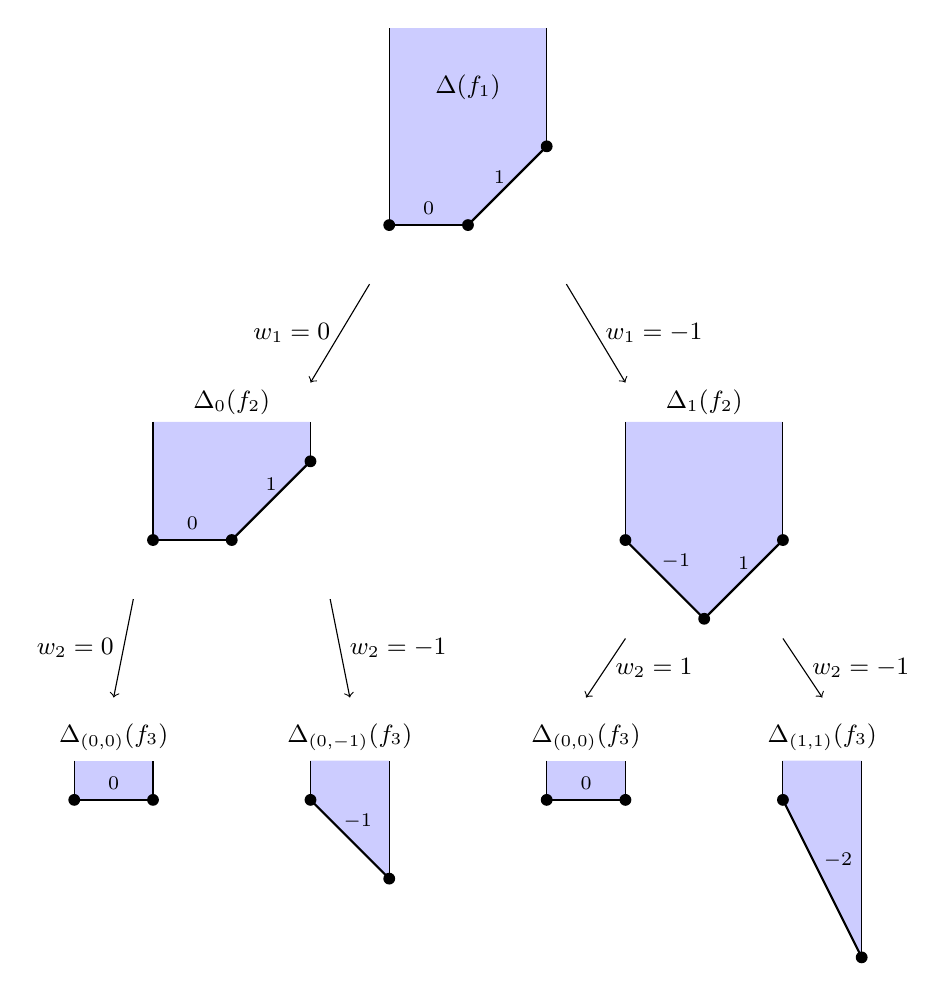
\begin{tikzpicture}
    % first level
    \fill[blue!20] (-1,2.5) -- (-1,0) -- (0,0) -- (1,1) -- (1,2.5) -- cycle;
    \draw (-1,2.5) -- (-1,0)
    (1,1) -- (1,2.5);
    \draw[thick,black]
      (-1,0) -- node[above,black,font=\scriptsize] {$0$} (0,0);
    \draw[thick,black]
      (0,0) -- node[anchor=south east,xshift=0.1cm,yshift=-0.1cm,black,font=\scriptsize] {$1$} (1,1);
    \fill (-1,0) circle (0.075cm);
    \fill (0,0) circle (0.075cm);
    \fill (1,1) circle (0.075cm);
    \node[font=\small] at (0,1.75) {$\Delta(f_1)$};

    \draw[->,black] (-1.25,-0.75) --
      node[left,black,font=\small] {$w_1=0$} ($(-1.25,-0.75)+(-0.75,-1.25)$);
    \draw[->,black] (1.25,-0.75) --
      node[right,black,font=\small] {$w_1=-1$} ($(1.25,-0.75)+(0.75,-1.25)$);

    % second level
    \node (o11) at (-3,-4) {};
    \fill[blue!20] ($(-1,1.5)+(o11)$) -- ($(-1,0)+(o11)$) -- ($(0,0)+(o11)$)
      -- ($(1,1)+(o11)$) -- ($(1,1.5)+(o11)$) -- cycle;
    \draw ($(-1,1.5)+(o11)$) -- ($(-1,0)+(o11)$)
      ($(1,1)+(o11)$) -- ($(1,1.5)+(o11)$);
    \draw[thick,black]
      ($(-1,0)+(o11)$) -- node[above,black,font=\scriptsize] {$0$} ($(0,0)+(o11)$);
    \draw[thick,black]
      ($(0,0)+(o11)$) -- node[above,black,font=\scriptsize] {$1$} ($(1,1)+(o11)$);
    \fill ($(-1,0)+(o11)$) circle (0.075cm);
    \fill ($(0,0)+(o11)$) circle (0.075cm);
    \fill ($(1,1)+(o11)$) circle (0.075cm);
    \node[font=\small] at ($(0,1.75)+(o11)$) {$\Delta_0(f_2)$};

    \draw[->,black] ($(-1.25,-0.75)+(o11)$) --
      node[left,black,font=\small] {$w_2=0$} ($(-1.25,-0.75)+(-0.25,-1.25)+(o11)$);
    \draw[->,black] ($(1.25,-0.75)+(o11)$) --
      node[right,black,font=\small] {$w_2=-1$} ($(1.25,-0.75)+(0.25,-1.25)+(o11)$);

    \node (o12) at (3,-4) {};
    \fill[blue!20] ($(-1,1.5)+(o12)$) -- ($(-1,0)+(o12)$) -- ($(0,-1) + (o12)$)
      -- ($(1,0)+(o12)$) -- ($(1,1.5)+(o12)$) -- cycle;
    \draw ($(-1,1.5)+(o12)$) -- ($(-1,0)+(o12)$)
      ($(1,0)+(o12)$) -- ($(1,1.5)+(o12)$);
    \draw[thick,black] ($(-1,0)+(o12)$) --
      node[above,black,font=\scriptsize,xshift=4pt] {$-1$} ($(0,-1)+(o12)$) --
      node[above,black,font=\scriptsize] {$1$} ($(1,0)+(o12)$);

    \fill ($(-1,0)+(o12)$) circle (0.075cm);
    \fill ($(0,-1)+(o12)$) circle (0.075cm);
    \fill ($(1,0)+(o12)$) circle (0.075cm);
    \node[font=\small] at ($(0,1.75)+(o12)$) {$\Delta_1(f_2)$};

    \draw[->,black] ($(-1,-1.25)+(o12)$) --
      node[right,black,font=\small] {$w_2= 1$} ($(-1.5,-0.75)+(0,-1.25)+(o12)$);
    \draw[->,black] ($(1,-1.25)+(o12)$) --
      node[right,black,font=\small] {$w_2= -1$} ($(1.5,-0.75)+(0,-1.25)+(o12)$);

    % third level
    \node (o21) at ($(o11)+(-2,-3.3)$) {};
    \fill[blue!20] ($(0,0.5)+(o21)$) -- ($(0,0)+(o21)$) -- ($(1,0)+(o21)$) -- ($(1,0.5)+(o21)$) -- cycle;
    \draw ($(0,0.5)+(o21)$) -- ($(0,0)+(o21)$)
      ($(1,0)+(o21)$) -- ($(1,0.5)+(o21)$);
    \draw[thick,black]
      ($(0,0)+(o21)$) -- node[above,black,font=\scriptsize] {$0$} ($(1,0)+(o21)$);
    \fill ($(0,0)+(o21)$) circle (0.075cm);
    \fill ($(1,0)+(o21)$) circle (0.075cm);
    \node[font=\small] at ($(0.5,0.8)+(o21)$) {$\Delta_{(0,0)}(f_3)$};

    \node (o22) at ($(o11)+(1,-3.3)$) {};
    \fill[blue!20] ($(0,0.5)+(o22)$) -- ($(0,0)+(o22)$) -- ($(1,-1)+(o22)$) -- ($(1,0.5)+(o22)$) -- cycle;
    \draw ($(0,0.5)+(o22)$) -- ($(0,0)+(o22)$)
      ($(1,-1)+(o22)$) -- ($(1,0.5)+(o22)$);
    \draw[thick,black]
      ($(0,0)+(o22)$) -- node[above,black,font=\scriptsize,xshift=0.1cm] {$-1$} ($(1,-1)+(o22)$);
    \fill ($(0,0)+(o22)$) circle (0.075cm);
    \fill ($(1,-1)+(o22)$) circle (0.075cm);
    \node[font=\small] at ($(0.5,0.8)+(o22)$) {$\Delta_{(0,-1)}(f_3)$};

    \node (o23) at ($(o12)+(-2,-3.3)$) {};
    \fill[blue!20] ($(0,0.5)+(o23)$) -- ($(0,0)+(o23)$) -- ($(1,0)+(o23)$) -- ($(1,0.5)+(o23)$) -- cycle;
    \draw ($(0,0.5)+(o23)$) -- ($(0,0)+(o23)$)
      ($(1,0)+(o23)$) -- ($(1,0.5)+(o23)$);
    \draw[thick,black]
      ($(0,0)+(o23)$) -- node[above,black,font=\scriptsize] {$0$} ($(1,0)+(o23)$);
    \fill ($(0,0)+(o23)$) circle (0.075cm);
    \fill ($(1,0)+(o23)$) circle (0.075cm);
    \node[font=\small] at ($(0.5,0.8)+(o23)$) {$\Delta_{(0,0)}(f_3)$};

    \node (o24) at ($(o12)+(1,-3.3)$) {};
    \fill[blue!20] ($(0,0.5)+(o24)$) -- ($(0,0)+(o24)$) -- ($(1,-2)+(o24)$) -- ($(1,0.5)+(o24)$) -- cycle;
    \draw ($(0,0.5)+(o24)$) -- ($(0,0)+(o24)$)
      ($(1,-2)+(o24)$) -- ($(1,0.5)+(o24)$);
    \draw[thick,black]
      ($(0,0)+(o24)$) -- node[above,black,xshift=0.2cm,font=\scriptsize] {$-2$} ($(1,-2)+(o24)$);
    \fill ($(0,0)+(o24)$) circle (0.075cm);
    \fill ($(1,-2)+(o24)$) circle (0.075cm);
    \node[font=\small] at ($(0.5,0.8)+(o24)$) {$\Delta_{(1,1)}(f_3)$};
  \end{tikzpicture}
  \caption{Series of Newton polygons of $F$ \cite[Figure~2]{tropPointsLinks}}
  \label{fig:seriesOfNewtonPolygons}
\end{figure}

With the ability to efficiently compute tropical varieties of zero-dimensional ideals we
can now focus on the central elements of fan traversals: Computing non-trivial points on a
tropical variety to find a starting cone and computing tropical links to determine
neighboring cones.

Finding non-trivial points on the tropical variety is achieved by intersecting with
sufficiently generic hyperplanes until the variety is zero-dimensional, allowing us to
apply Algorithm~\ref{alg:zeroDimTrop}. But when is a point non-trivial? For an ideal $I
\idealof K[\vec x]$ we define the \emph{homogeneity space} of $I$ to be the linear
subspace
\[
  C_0(I) = \left\{ \vec w \in \setR^n : \initial_{\vec w}(I) = I \right\}.
\]
It can be computed easily from any reduced Gröbner basis for $I$ and is trivially included
in $\Trop(I)$ if $I$ itself contains no monomial. In fact, $C_0(I)$ is contained in every
cone of the tropical variety, so computing a point in the homogeneity space offers no
useful information for our algorithms. Hence, we call a point $\vec w \in \Trop(I)$
\emph{non-trivial} if $\vec w \not\in C_0(I)$. The following proposition formalizes the
process of intersecting with generic hyperplanes:

\begin{proposition}
  Let $I \idealof K[\vec x]$ be an ideal of dimension $\dim I = d$ with algebraically
  independent set $\{x_1, \dots, x_d\}$ and suppose its affine variety $X := V(I)$
  satisfies $X \cap \setT^n \neq \varnothing$. Then there exists an non-empty Zariski-open
  subset $U \subseteq \setT^d$ such that for all $\lambda \in U$
  \[
    \varnothing \neq X_\lambda :=
    X \cap V(x_1-\lambda_1, \dots, x_d - \lambda_d) \subseteq \setT^n
  \]
  and $\dim X_\lambda = 0$.
  \label{prp:intersHyperp}
\end{proposition}

The resulting algorithm then just uses that by Theorem~\ref{thm:tropComplexConn} the
maximal cones in the tropical variety have the same dimension as the defining ideal and
puts Proposition~\ref{prp:intersHyperp} to work:

\begin{algo}[Tropical Points, {\cite[Algorithm~3.3]{tropPointsLinks}}] $ $
  \begin{algorithmic}[1]
    \Require $I \idealof K[\vec x]$,
    \Ensure $\vec w \in \Trop(I) \setminus C_0(I)$.
    \State Compute a maximal algebraically independent set, say $\{x_1, \dots, x_d\}$ and
    the homogeneity space $C_0(I)$.
    \Repeat
      \State Pick $\vec w \in \setQ^d$ random with $\{\vec w\} \times \setR^{n-d} \cap
        C_0(I) = \varnothing$.
      \State Pick $c \in K^d$ random with $\nu(c) = \vec w$.
      \State Set $I_c := I|_{x_i = c_i} \idealof K[x_{d+1}, \dots, x_n]$
    \Until{$\dim(I_c) = 0$ and $V(I_c) \subseteq \setT^{n-d}$}
    \State Compute a triangular set $F$ with $I_c \subseteq \ideal F$.
    \State Compute $(w_{d+1}, \dots, w_n) \in \Trop(F)$ using
      Algorithm~\ref{alg:zeroDimTrop}.
    \State\textbf{return} $(w_1, \dots, w_d, w_{d+1}, \dots, w_n)$.
  \end{algorithmic}
  \label{alg:tropicalPoint}
\end{algo}

We previously did not specify how to compute an initial starting cone for
Algorithm~\ref{alg:traversal}. Computing the maximal Gröbner cone $C_{\vec w}(I)$ (resp.\
the corresponding pair of reduced Gröbner bases) containing the point $\vec w$ in its
relative interior will yield a suitable starting cone.

\begin{example}
  % TODO
  We now apply this procedure to find a non-trivial point of \dots% TODO
\end{example}

% TODO write differently from source?
To conclude this section we want study an alternative method of obtaining points in
neighboring cones. We call a tropical variety $\Trop(I)$ a \emph{tropical curve} if it is
one dimensional and say it is \emph{combinatorially a curve} if $\Trop(I)/C_0(I)$ is
one-dimensional. Then, for any $\vec u \in \Trop(I)$ sitting in the relative interior of a
cell of codimension one, that is, a facet of some maximal cone, we call
$\Trop(\initial_{\vec u}(I))$ the \emph{tropical link} of $I$ around $\vec u$. This set is
the support of a polyhedral fan, since it is a tropical variety, and also combinatorially
a curve which describes $\Trop(I)$ locally around $\vec u$. This was shown in the proof of
the correctness of \cite[Algorithm~4.10]{compTropVar}. The properties needed for our
algorithm are as follows, mainly due to \cite{ossTropLift}

\begin{thmCorollary} \label{thmc:tropInt}
  Let $X$ and $X$ be two affine subvarieties. If the intersection $\Trop(X) \cap
  \Trop(X')$ has codimension $\codim\Trop(X) + \codim\Trop(X')$ in a neighborhood of $\vec
  w$, then $\vec w \in \Trop(X\cap X')$. In particular:
  \begin{enumerate}
    \item Assume $\Trop(I)$ is combinatorially a curve with $\dim C_0(I) = d$ and
      $C_0(I)\cap \Lin(e_{d+1}, \dots, e_n) = \{0\}$, then for any $c \in \setT^d$ we have
      \[
        \Trop(I) \cap \{\nu(c)\} \times \setR^{n-d} = \Trop(I + \ideal{x_1-c_1, \dots,
        x_d-c_d}),
      \]
      and this tropical variety is a tropical curve.
      \label{thmc:i}
    \item If $\Trop(I)$ is a one-dimensional polyhedral fan, then for any $c \in K^* =
      \setT^1$ with $\nu(c)\neq0$ we have
      \[
        \Trop(I) \cap \{\nu(c)\} \times \setR^{n-1} = \Trop(I + \ideal{x_1-c_1})
      \]
      and this tropical variety is zero-dimensional.
      \label{thmc:ii}
  \end{enumerate}
\end{thmCorollary}

Finally, the structure of the tropical combinatorial curves $\Trop(\initial_{\vec w}(I))$ together
with the above corollaries culminate in the following algorithm:

\begin{algo}[Tropical Links, {\cite[Algorithm~4.5]{tropPointsLinks}}]\
  \label{alg:tropLinks}
  \begin{algorithmic}[1]
    \Require $I \idealof K[\vec x]$ such that $\Trop(I)$ is combinatorially a curve and a
    polyhedral fan,
    \Ensure $W \subseteq \setR^n$ such that $\Trop(I) = \bigcup_{\vec w \in W} \vec w
      \cdot \setR_{\geq0} + C_0(I)$
    \State Suppose $\dim C_0(I) = d$ and assume w.l.o.g. $C_0(I) \cap \Lin(e_{d+1}, \dots,
      e_n) = \{0\}$.
    \State Let $J \idealof K[x_d, \dots, x_n]$ be the image of $I$ under the substitution
      map
      \[
        K[x_1, \dots, x_n] \to K[x_d, \dots, x_n], x_i \mapsto
        \begin{cases}
          t, & \text{if } i < d, \\
          x_i & \text{else},
        \end{cases}
      \]
      where $t \in K$ is a fixed uniformizing parameter.
      \label{alg:links:cut}
    \For{$i = d, \dots, n$}
      \State Let $J_i^\pm$ be the images of $J$ under the maps $x_i \mapsto t^\pm$
        respectively,
        \label{alg:links:curve}
      \State Compute $V_i^\pm = \Trop(J_i^\pm)$ using Algorithm~\ref{alg:zeroDimTrop},
      \State Set
        \begin{align*}
          W_i^\pm := \Bigl\{
            &(1, \dots, 1, w_d, \dots, w_{i-1}, \pm1, w_{i+1}, \dots, w_n) : \\
            &(w_d, \dots, w_{i-1}, w_{i+1}, \dots, w_n) \in V_i^\pm
          \Bigr\} \subseteq \setR^n
        \end{align*}
      \State Scale elements of $W_i^\pm$ positively until they are primitive in $\setZ^n$.
    \EndFor
    \State Set $W = \bigcup_{i=d}^n (W_i^+ \cup W_i^-)$.
    \State\textbf{return} $W$.
  \end{algorithmic}
\end{algo}

Indeed, the steps above are just applying the Corollaries~\ref{thmc:tropInt} for every
remaining dimension: In line~\ref{alg:links:cut} we cut the combinatorial curve down to an
actual tropical curve by Corollary~\ref{thmc:tropInt}.\ref{thmc:i}. Then in
line~\ref{alg:links:curve} we consider the respective zero-dimensional varieties described
in \ref{thmc:tropInt}.\ref{thmc:ii}. Note that, since a tropical curve is the support
of a tropical fan in this setting, it is necessarily a collection of rays. Hence the
representation as $\bigcup_{w \in W} w\cdot \setR_{\geq0} + C_0(I)$ is justified. This
algorithm can then be used in line \ref{alg:interiorPoints} of
Algorithm~\ref{alg:neighbors} as a replacement for the methods concerning prevarieties. As
the timings in \cite{tropPointsLinks} show, this offers a considerable speedup in general.

\section{Parallelization}

Our main contribution is the combination of \textsc{Singular}-methods to compute tropical
varieties with recently developed parallelization efforts at the Fraunhofer ITWM of
computer algebra software. The first efforts to this end are described in
\cite{towardsParallel} while we specifically base our work on parallelization algorithms
by Christian Reinbold to compute GIT-fans (cite???). Parallelization of our procedures is
taken care of by the GPI-Space environment:

Use Petri nets as a framework to parallelize the traversal of tropical fans. Refer to
source \cite{towardsParallel}.
% TODO write more introduction

\subsection{Petri Nets and GPI-Space}

Petri nets are used as a coordination language in GPI-Space, which allow us to formulate
our algorithms without explicitly specifying any parallelization. Further, they can be
expressed as bipartite directed graphs, allowing them to be designed in an intuitive and
accessible way.

\begin{definition}[Petri net]
  \label{def:petri}
  A \emph{Petri net} is a triple $N = (P, T, F)$ of two disjoint finite sets $P$ and $T$
  called \emph{places} and \emph{transitions} respectively and a subset $F \subseteq
  (P\times T) \cup (T \times P)$ called the \emph{flow relation} of the net.
\end{definition}

This definition establishes the static part of a Petri net which is used to describe the
overall structure of a program. To describe the dynamic execution of a Petri net we
introduce the notion of markings:

\begin{definition}[Marking]
  \label{def:marking}
  Given a Petri net $(P,T,F)$ a \emph{marking} $M$ of the net is defined as a function $M
  : P \to \setN$. If $M(p) = k$ for some $k \in \setN$ then we say that $p$ \emph{holds
  $k$ tokens under $M$}.
\end{definition}

As we will be using Petri nets with markings to formulate program flows to parallelize, it
makes sense to think of transitions as the elementary algorithms with tokens representing
the data which is passed from and to these algorithms. Thus we will call $p$ an
\emph{input} to $t$ if $(p,t) \in F$ and analogously an \emph{output} to $t$ if $(t,p) \in
F$.

We can also describe a marking by its graph $M = \{ (p, M(g)) : p \in P, M(g) \neq 0 \}$
of non-zero images. Such a marking $M$ is used to define the \emph{state} a Petri net: $M$
\emph{enables} a transition $t \in T$ if all input places of $t$ hold tokens, meaning that
$(p,t) \in F$ implies $M(g)>0$. In this case we write $\smash{M
\overset{t}{\longrightarrow}}$. In a Petri net with marking $M$ a transition $t$ enabled
by $M$ may be \emph{fired} by consuming a token from each input place of $t$ and adding a
token to each output place. This leads to a new marking $M'$ given by
\[
  M'(p) = M(p) - |\{ (p,t) \} \cap F| + |\{ (t,p) \} \cap F|
\]
for all $p \in P$. If $M'$ is defined in this way by firing $t$, then we write $\smash{M
\overset{t}\longrightarrow M'}$ and say that $M'$ is \emph{directly reachable} from $M$ by
firing $t$. In general we say that a marking $M'$ is \emph{reachable} if there is a
\emph{firing sequence} $\smash{M \overset{t_1}\longrightarrow M_1
\overset{t_2}\longrightarrow \cdots \overset{t_{n-1}}\longrightarrow M'}$. It is important
to note that the firing of enabled places is a local process, that is, it does not block
other enabled transitions from firing as well. This is the most important property
allowing parallelisms.
% TODO more on reachabiliy?

A nice property of Petri nets is that their static part given by
Definition~\ref{def:petri} can be visualized as a directed bipartite graph. Recall that a
directed graph $G = (V,E)$ is \emph{bipartite} is there is some partition $V = V_1 \dotcup
V_2$ of the node set such that $E \subseteq (V_1 \times V_2) \cup (V_2 \cup V_2)$, meaning
no arc connects nodes lying in the same set $V_i$. But by definition of the Petri net
$(P,T,F)$ this clearly holds for the graph $G = (P \cup T, F)$ where we interpret places
and transitions as nodes and their flow relations as arcs. This will be illustrated in the
upcoming examples, see for instance figure~\ref{fig:petriEx}. Usually, places will be
represented by circles and transitions as boxes, while tokens held by places will be drawn
as points in the corresponding place. We will also mark places or transitions with letters
if necessary.

\begin{figure}[htbp]
  \centering
  \begin{subfigure}{.35\textwidth}
    \centering
    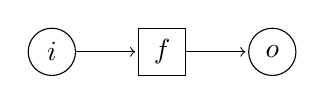
\begin{tikzpicture}[node distance=1.4cm]
      \node [place]      (in)                {$i$};
      \node [transition] (f)   [right of=in] {$f$} edge [pre] (in);
      \node [place]      (out) [right of=f]  {$o$} edge [pre] (f);
    \end{tikzpicture}
    \caption{Data parallelism}
    \label{fig:petri:datapar}
  \end{subfigure}
  \begin{subfigure}{.64\textwidth}
    \centering
    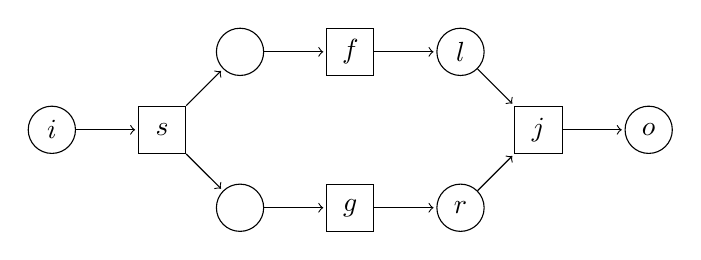
\begin{tikzpicture}[node distance=1.4cm]
      \node [place]      (in) {$i$};
      \node [transition] (s)  [right of=in] {$s$} edge [pre] (in);

      \node [place]      (su) [above right of=s] {}    edge [pre] (s);
      \node [transition] (f)  [right of=su]      {$f$} edge [pre] (su);
      \node [place]      (l)  [right of=f]       {$l$} edge [pre] (f);

      \node [place]      (sd) [below right of=s] {}    edge [pre] (s);
      \node [transition] (g)  [right of=sd]      {$g$} edge [pre] (sd);
      \node [place]      (r)  [right of=g]       {$r$} edge [pre] (g);

      \node [transition] (j)  [below right of=l] {$j$} edge [pre] (l) edge [pre] (r);
      \node [place]      (o)  [right of=j]       {$o$} edge [pre] (j);
    \end{tikzpicture}
    \caption{Task parallelism}
    \label{fig:petri:taskpar}
  \end{subfigure}
  \caption{Petri nets illustrating parallelisms}
  \label{fig:petriEx}
\end{figure}

\begin{example}[Parallelisms in Petri Nets]
  \label{ex:petriPar}
  We now want to look at how different kinds of parallelisms can be realized in Petri
  nets.
  \begin{enumerate}[label=(\alph*)]
    \item First consider the Petri net $\Psi = (P,T,F)$ given by $P = \{i, o\}$, $T =
      \{f\}$ and $T = \{ (i,f), (f,o) \}$ whose graph is depicted in
      figure~\ref{fig:petri:datapar}. Let $M=M_0 = \{ (i, n) \}$ be the initial marking
      for some $n>1$, then the transition $f$ is enabled. Firing $f$ once yields the new
      marking $M_1 = \{ (i, n-1), (o, 1) \}$, so $t$ is still enabled. Hence $f$ may fire
      $n-1$ more times, yielding the marking $M' = M_n = \{ (o,n) \}$, which we usually
      denote by $\smash{M \overset{t^n}{\longrightarrow} M'}$. As there is no
      interdependence between the tokens held in $i$ the transition $f$ may fire for each
      one at the same time. This form of parallelism is then used in GPI-Space, as firing
      transitions will not be an immediate change in most real world applications.
      Applying a function or procedure to several inputs is precisely \emph{data
      parallelism}: We may regard each token in $i$ as a part of a larger chunk of data
      that is fed to $f$. Note that we will introduce tokens which hold actual data later
      on.
      % TODO
    \item Consider now the Petri net given by the graph depicted in
      figure~\ref{fig:petri:taskpar}. If we start with the marking $M = \{ (i,1) \}$, then
      firing $s$ will enable both $f$ and $g$. Both of these transitions may thus fire in
      parallel.
      % TODO
  \end{enumerate}
\end{example}

To summarize, Petri nets contain information about \emph{all} activities that may be
executed at any given time, making it possible to exploit the maximum amount of
parallelism. But as was hinted at above, Petri nets in the current form are not yet
suitable to model algorithms together with the data they produce as they arise from real
world applications.

% TODO GPI-Space

\subsection{Traversing a Fan in Parallel}
\label{sec:traverseParal}

Computing tropical varieties in our setting follows the general structure of a fan
traversal: Interpreting the maximal cones of a polyhedral fan together with their
adjacency relations as a connected graph, we may realize the fan traversal as a simple
graph traversal. To this end we want to formulate the version of
Algorithm~\ref{alg:traversal} enhanced with Algorithm~\ref{alg:tropLinks} into a Petri
net. Indeed on first glance an implementation looks quite simple: After determining a
starting cone using Algorithm~\ref{alg:tropicalPoint} we construct a set of
\emph{unprocessed} and \emph{processed} cones respectively. However, these steps alone do
not suffice quite yet: Recall that transitions do not in general fire instantaneously, so
there might be situations where the set of unprocessed cones might be empty, while some
transitions still process data. It is thus important to devise proper termination
conditions to properly stop the execution of the net. Before we can tackle this problem we
must consider some implementation details first that will be reflected in the description
of our algorithm.
\begin{enumerate}[label=\arabic*.]
  \item We must first decide how to store and represent input and intermediate results.
    Each Gröbner cone is represented by a pair of Gröbner bases and usually we add the
    actual cone obtained from them to the data as well. Further, we require the ambient
    polynomial ring in which the corresponding ideals live as they contain the information
    about the term ordering. Also, it is not possible to store an ideal without also
    storing its ambient ring in \textsc{Singular}. As it turns out, the inbuilt storage
    solutions in the GPI-Space environment are not suitable to handle the amount of data
    that is exchanged between processes. Instead we use a separate storage solution that
    will be accessed by the GPI-Space environment. We will discuss implementation details
    hereof in the next section.
  \item We previously noted that it is necessary to be able to test two given Gröbner
    cones for equality. While we may compare the given initial ideals as they cannot
    differ by definition, it is faster to instead consider the actual cones. If they are
    given in canonical form, we may associate a \emph{unique point} to each of them. It is
    then sufficient to compare the unique points with each other. The unique point may
    then also be used as a \emph{key} for storage purposes.
    % TODO more?
  \item Finally, in the context of tropical varieties it is desirable to consider the
    corresponding polyhedral fan modulo symmetry. More precisely, for a polyhedral fan
    $\mathcal F$ in $\setR^n$ we want to find a subgroup of permutations $G \leq S_n$
    that acts trivially on $\mathcal F$ but produces non-trivial cone orbits. It turns out
    that considering the cones modulo symmetry is compatible with how their unique points
    are computed, so we additionally get orbits of unique points. As these are just
    integer vectors, we even pick a minimal representative by sorting lexicographically.
    This allows to compare cones under symmetry very quickly.
\end{enumerate}
From now on, we want to successively construct a Petri net describing our traversal
algorithm. However, Algorithm~\ref{alg:traversal} is not yet formulated in a way that is
suitable to parallelize. We give a slight reformulation and add the computation of a
starting pair of Gröbner bases.

\begin{algo}[Traversal (Modified)]\
  \label{alg:traversalMod}
  \begin{algorithmic}[1]
    \Require A (homogeneous) prime ideal $I \idealof K[\vec x]$ and a symmetry group $G$
      as above.
    \Ensure The set of maximal Gröbner cones of the polyhedral fan whose support is
      $\Trop(I)$ (resp.\ the corresponding pairs of Gröbner bases).
    \State Compute a $\vec w \in \Trop(I) \setminus C_0(I)$ using
      Algorithm~\ref{alg:tropicalPoint}.
    \State Compute the pair $c_0 := (\mathcal G_{\prec_{\vec w}}(\initial_{\vec w}(I)),
      \mathcal G_{\prec_{\vec w}}(I))$ from $I$ and $\vec w$.
    \State Set $U = \{ c_0 \}$ and $P = \varnothing$.
    \While{$U \neq \varnothing$}
      \State Pick a pair of Gröbner bases $c \in U$.
      \If{$c \not\in P$} \label{alg:line:coneExists}
        \State Compute $N = \mathrm{Neighbors}(c)$ using Algorithm~\ref{alg:neighbors}
          enhanced by Algorithm~\ref{alg:tropLinks}.
        \State Set $U = U \setminus \{ c \} \cup N$, $P = P \cup \{ c \}$.
      \EndIf
    \EndWhile
    \State\textbf{return} $P$.
  \end{algorithmic}
\end{algo}

Note that we check in line~\ref{alg:line:coneExists} for existence with respect to the
symmetry group $G$, so if $\{ \id \} \lneq G$ it is possible that we discard cones which
were not found yet themselves, but lie in the orbit of some cone in $P$. This will become
important later on again when we further refine this algorithm.

\begin{figure}[tbhp]
  \centering
  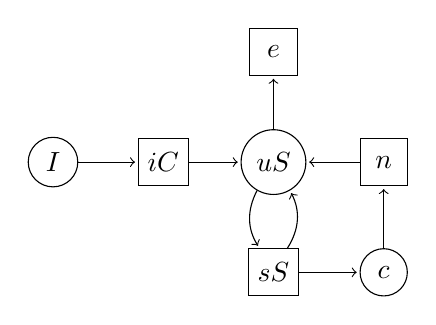
\begin{tikzpicture}[node distance=1.4cm]
    \node [place] (in) {$I$};
    \node [transition] (init) [right of=in] {$iC$} edge [pre] (in);

    \node [place] (unpList) [right of=init] {$uS$} edge [pre] (init);
    \node [transition] (split) [below of=unpList] {$sS$}
      edge [pre, bend left]   (unpList)
      edge [post, bend right] (unpList);
    \node [place] (cone) [right of=split] {$c$}
      edge [pre] (split);
    \node [transition] (neigh) [right of=unpList] {$n$}
      edge [pre] (cone)
      edge [post] (unpList);
    \node [transition] (e) [above of=unpList] {$e$} edge [pre] (unpList);
  \end{tikzpicture}
  \caption{Naive approach to traversing a polyhedral fan}
  \label{fig:naive}
\end{figure}

In figure~\ref{fig:naive} we see a first sketch of what a possible formulation could look
like but note that no termination logic has been included yet. The net is executed as
follows:
\begin{itemize}
  \item It is initialized with a single token on the place $I$ which holds the pair $(I,
    G)$ for the prime ideal $I$ and its symmetry group $G$.
  \item The transition $iC$ consumes this token and computes an initial starting cone
    given as a triple
    \[
      c_{\vec w} = (
        \mathcal G_{\prec_{\vec w}}(\initial_{\vec w}(I)),
        \mathcal G_{\prec_{\vec w}}(I),
        C_{\vec w}(I)
      )
    \]
    of reduced Gröbner bases and their corresponding Gröbner cone. Afterwards, $iC$
    produces a token holding the datum $\{c_{\vec w}\}$.
  \item The place $uS$ holds tokens with \emph{sets} (or lists) of these triples as their
    data, which we interpret as the \emph{unprocessed} cones. For a token in $uS$ there is
    two cases for the set $\mathcal C$ it holds: It is the empty set or it contains a
    non-zero amount of Gröbner cone triples:
    \begin{itemize}
      \item If the token holds the empty set, then it will be consumed by the transition
        $e$ which does nothing else.
      \item Otherwise we may pick a $c_{\vec w} \in \mathcal C$. The transition $sS$
        consumes the token holding $\mathcal C$, pushes back $\mathcal C\setminus \{
        c_{\vec w}\}$ to $uS$ and pushes $c_{\vec w}$ to the place $c$.
    \end{itemize}
    In short, the transition $sS$ processes sets of triples into tokens of single triples.
  \item Finally, the transition $n$ consumes tokens from $c$ which holds the Gröbner cone
    triples and applies the modified neighbor algorithm to them. Accordingly it produces
    sets of such triples which are then pushed to $uS$.
\end{itemize}
Note that for this to make sense we have to assume that the transition $n$ stores and has
access to the processed Gröbner cones and thus only pushes \enquote{new} cones onto the
place $uS$. As said above this net does not contain any termination logic and is thus not
complete. One way to properly terminate if and only if no more neighbors can be found is
to keep track of the number of all tokens that hold unprocessed cones, including those
that are being processed. If this number drops to zero while all the places $sS$ and $c$
hold no tokens then the algorithm can terminate.

% TODO explain read only ports
\begin{figure}[tbhp]
  \centering
  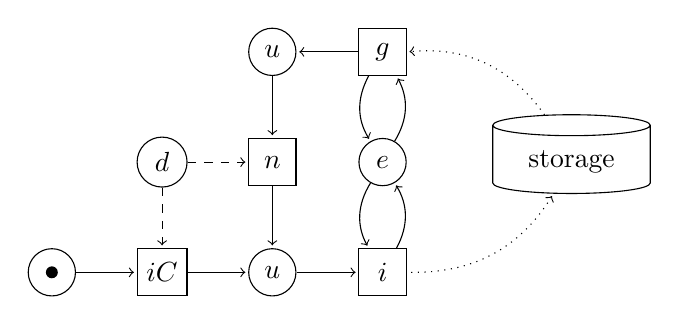
\begin{tikzpicture}[node distance=1.4cm]
    \node [place,tokens=1] (ctrl) {};
    \node [transition] (init) [right of=ctrl] {$iC$} edge [pre] (ctrl);

    \node [place] (unproc) [right of=init] {$u$} edge [pre] (init);
    \node [transition] (insert) [right of=unproc] {$i$} edge [pre] (unproc);
    \node [transition] (neighbors) [above of=unproc] {$n$} edge [post] (unproc);
    \node [place] (unprocCones) [above of=neighbors] {$u$} edge [post] (neighbors);
    \node [transition] (get) [right of=unprocCones] {$g$} edge [post] (unprocCones);

    \node [place] (enabled) [below of=get] {$e$}
      edge [post,bend right] (get)
      edge [pre,bend left] (get)
      edge [post,bend right] (insert)
      edge [pre,bend left] (insert);

    \node [database] (stor) [right of=enabled,xshift=1cm] {storage}
      edge [bend right,dotted,post] (get)
      edge [bend left,dotted,pre] (insert);

    \node [place] (data) [above of=init] {$d$}
      edge [post,dashed] (init)
      edge [post,dashed] (neighbors);
  \end{tikzpicture}
  \caption{Slightly less naive approach incorporating external storage}
  \label{fig:naive:storage}
\end{figure}

Note that the algorithm given above is just a general graph traversal algorithm where $iC$
provides the starting node and $n$ provides neighboring nodes. Before we want to exploit
some properties specific to tropical varieties we have to incorporate the above storage
plans into our Petri net. This new version is depicted in Figure~\ref{fig:naive:storage}
and works much in the same way:
\begin{itemize}
  \item The transition $iC$ and $n$ are unchanged, take the same input and produce the
    same output as before, with one exception:
  \item The place $d$ holds the data $(I, G)$ and is read-only. Hence $iC$ fires by
    consuming the control token that was added. By initializing this place with exactly
    one token, we ensure that the initial Gröbner cone is computed exactly once. In the
    previous Petri net we implicitly assumed that $G$ is part of the tokens that are fed
    to $n$.
  \item Similarly, $u$ holds sets the unprocessed Gröbner cone triples produced by $iC$
    and $n$.
  \item The $i$ and $g$ transitions \emph{insert} and \emph{get} tokens of Gröbner cone
    sets respectively. For this they call retrieval and insertion operations provided by
    the external storage interface. Note that, as we may insert sets, this removes the
    need for the splitting operations by $sS$ in the previous net.
    % TODO!!!
\end{itemize}

% TODO

\subsection{Adaptation and Implementation Details}

As was previously mentioned we heavily rely on work done by Christian Reinbold on
GIT-fans \cite{reinboldGitFan}. His work, in turn, relies on work done by Lukas Ristau to
enable a seamless integration into a GPI-Space project.

Introduce GIT-fans as similarly structured object

Adapting existing code base

Make in particular use of termination logic -- not trivial!

\section{Performance and Scalability}

In this section we want to apply our implemented algorithms to real world examples in
order to examine how efficient they parallelize. The idea is to consider examples which
are \enquote{big} enough to provide reliable parallelization timings. An important class
of (tropical) varieties already considered in \cite{tropPointsLinks} and \cite{tropGrass}
are the so-called \emph{tropical Grassmannians} which can be parameterized to arbitrary
dimensions. We want to compare the single-threaded computing times of the
\textsc{Singular}-only version of our algorithm with the parallel version by considering
the tropical Grassmannian $\mathcal G_{3,7}$. While this tropical variety is sufficiently
small to be computed successfully on any private machine, we also want to consider
examples which have not been computed in their entirety before. An example for this is the
much larger tropical Grassmannian $\mathcal G_{3,8}$.

Our running time test were executed on the cluster computing provided by Fraunhofer ITWM
in Kaiserslautern. This cluster is comprised of 192 computing nodes each fitted with 16
Intel Xeon E5-2670 processor cores running at 2.6 GHz with 64\,GB memory. The GPI-Space
engine uses these cores without hyperthreading, meaning we may run a maximum of 16 jobs
per node. The nodes are connected via FDR Infiniband.

\subsection{Tropical Grassmannians}

One important class of tropical varieties are the tropical Grassmannians which arise as
the tropical varieties of the equally -- if not more -- important Grassmannians which can
be interpreted as projective varieties. Some results on the tropical Grassmannian can be
found in \cite{tropGrass}.

\begin{definition}[Grassmannians]
  Let $n \in \setN_{>0}$ and $k \in \setN$ with $0 \leq k \leq n$, then the
  \emph{Grassmannian} of $k$-planes in $K^n$ is the set of all $k$-dimensional linear
  subspaces of $K^n$, usually denoted by $\Grass(k, n)$.
\end{definition}

Thus, Grassmannians are in some sense a generalization of projective space: for instance
we will later be able to see that in fact $\Grass(1,n) \cong \setP^n$. Our goal now is to
give these sets the structure of a projective variety which in turn allows us to study
their tropical variety. This is achieved by embedding a Grassmannian $\Grass(k, n)$ into
$\setP^{\binom nk}-1$ via the so-called \emph{Plücker embedding}. To this end we want to
regard the corresponding linear spaces as elements of projective space, which first
requires some constructions from commutative algebra.

Let $V$ and $W$ be two vector spaces and $k\in\setN$, then a multilinear map $f : V^k \to
W$ is called \emph{alternating} if for all $v_1, \dots, v_k$ with $v_i=v_j$ for some
distinct $i,j$ we have that $f(v_1, \dots, v_k) = 0$. In this setting an \emph{alternating
$k$-fold tensor product} of $V$ is a vector space $T$ together with an alternating map
$\wedge:V^k\to T, (v_1, \dots, v_k) \mapsto v_1\wedge\cdots\wedge v_k$ such that for any
other alternating map $f:W\to T$ there is a unique $\tilde f:T\to W$ satisfying $\tilde f
\circ \wedge = f$. It is easy to prove that such an alternating tensor product always
exists and is in fact unique up to isomorphism -- the proof is completely analogous to the
case of standard tensor products. Hence we may write $\bigwedge^k V := T$ for these vector
spaces. In the following we present some interesting and necessary properties of these
spaces which can be proved with basic knowledge of commutative algebra:

\begin{remark}
  Let $V$ be a vector space, $k \in \setN$ and $\bigwedge^k V$ the corresponding
  alternating tensor product.
  \begin{enumerate}
    \item If $v_1, \dots, v_n$ is a basis of $V$ where $n=\dim V$ as a $K$-vector space,
      then the set
      \[
        \left\{
          v_{i_1} \wedge \cdots \wedge v_{i_k} : 1\leq i_1 < \cdots < i_k \leq n
        \right\}
      \]
      will be a basis of $\bigwedge^kV$. In particular this vector space is of dimension
      $\dim\bigwedge^kV = \binom nk$.
    \item For elements $v_1, \dots, v_k \in V$ the \emph{pure tensor} $v_1\wedge \cdots
      \wedge v_k \in \bigwedge^kV$ will be non-zero if and only if $v_1, \dots, v_k$ are
      linearly independent in $V$.
    \item It follows that for two linear independent families $v_1, \dots, v_k, w_1,
      \dots, w_k \in V$ we have that $v\wedge\cdots \wedge v_k$ and $w_1\wedge\cdots\wedge
      w_k$ are linearly dependent if and only if the families both span the same linear
      subspace of $V$.
  \end{enumerate}
\end{remark}

Consider now our setting where $V=K^n$ and let $N = \smash{\binom nk}$ be the number of
basis elements in $\bigwedge^kK^n$. We may identify a $k$-dimensional linear subspace $X
\in \Grass(k,n)$ of $V$ with a pure tensor in $\bigwedge^kV \cong K^N$ uniquely up to
scalar multiplication which -- by definition -- makes the corresponding embedding
$\Grass(k,n) \to \setP^{N-1}$, called the \emph{Plücker embedding}, injective. Hence we
can regard $\Grass(k,n)$ as a subset of this projective space. Finally, to equip
$\Grass(k,n)$ with the structure of a projective variety, we need this fact: For non-zero
$w\in \bigwedge^kK^n$ the rank of the $K$-linear map $f:K^n \to \bigwedge^{k+1}K^n, v
\mapsto v \wedge w$ is at least $n-k$ and equality holds if and only if $w$ is a pure
tensor. Thus, using the above embedding, $\Grass(k,n)$ consists entirely of pure tensors
$w\in \Grass(k,n)$ which all define maps $v\mapsto v\wedge w$ of rank at most $n-k$. This
is equivalent to all $(n-k+1) \times (n-k+1)$-minors of these maps vanishing which induces
polynomial equations in the Plücker coordinates of $\setP^{N-1}$ describing $\Grass(k,n)$,
hence it is in fact a projective variety.

On an additional note one can cover $\Grass(k,n)$ with copies of $\setA^{k(n-k)}$ to show
that the Grassmannian is an irreducible projective variety of dimension $k(n-k)$. This
leads to the following definition:

\begin{definition}[Tropical Grassmannians]
  By the above a Grassmannian can be viewed as a projective variety given by a homogeneous
  prime ideal
  \[
    I(\Grass(k,n)) \idealof K[ p_{i_1, \dots, i_k} : 1\leq i_1 < \cdots < i_k \leq n ]
  \]
  with Plücker coordinates $p_{i_1,\dots,i_k}$ which defines a determinantal variety
  $\Grass(k, n)$. This, in turn, defines a tropical variety and we write $\mathcal G_{k,n}
  := \Trop(I(\Grass(k,n)))$.
\end{definition}

\begin{figure}[tbhp]
  \centering
  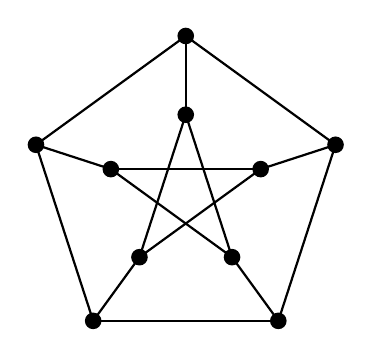
\begin{tikzpicture}[thick]
    \foreach \x in {0, 1, ..., 4}
    {
      \fill ({\x*72+90}:1) circle (3pt);
      \fill ({\x*72+90}:2) circle (3pt);
      \draw ({\x*72+90}:1) -- ({\x*72+90}:2);
      \draw ({\x*72+90}:1) -- ({\x*72+234}:1);
      \draw ({\x*72+90}:2) -- ({\x*72+162}:2);
    }
  \end{tikzpicture}
  \caption{Petersen graph illustrating connectivity of $\mathcal G_{2,5}$}
  \label{fig:petersen}
\end{figure}

\begin{example}\
  \begin{enumerate}
    \item As we clearly have $\Grass(0,n) \cong \Grass(n,n) \cong K^n$ and $\Grass(1,n)
      \cong \Grass(n-1, n) \cong \setP_K^{n-1}$, the first \enquote{non-trivial}
      Grassmannian is $\Grass(2,4)$. By the process described above one easily finds that
      $\Grass(2,4)$ is given by the ideal
      \[
        I_{2,4} := \ideal{ x_{i,j} \phi : 1 \leq i < j \leq 4 }
        \idealof K[x_{1,2}, \dots, x_{3,4}].
      \]
      for $\phi = x_{1,2}x_{3,4} - x_{1,3}x_{2,4} + x_{1,4}x_{2,3}$, but $\dim I_{2,4} =
      5$, so it defines a hypersurface in $\setP^5$. It can be shown that in fact
      $\sqrt{I_{2,4}} = \ideal \phi$, so $\Grass(2,4) = V(\phi)$ as one would expect.
      Hence the polyhedral fan corresponding to the tropical variety $\mathcal G_{2,4}$
      has maximal five-dimensional cones living in $\setR^6$.

      Computations show that $\mathcal G_{2,4}$ consists of three five-dimensional cones
      with four-dimensional homogeneity-space as their common facet. In particular,
      $\mathcal G_{2,4}$ is combinatorially a curve and $\mathcal G_{2,4}/C_0(\phi)$ is a
      tropical line consisting of three rays from the origin.
    \item The next non-trivial Grassmannian $\Grass(2,5)$ is given by five similar
      quadrics from the polynomial ring $K[x_{1,2}, \dots, x_{4,5}]$ in ten variables. Its
      tropical variety $\mathcal G_{2,5}$ is given by a seven-dimensional fan consisting
      of ten seven-dimensional cones and fifteen six-dimensional cones. Each maximal cone
      has three of the fifteen six-dimensional cones as facets. The homogeneity space
      $C_0(I_{2,5})$ is five-dimensional. Intersecting $\mathcal G_{2,5}/C_0(I_{2,5})$
      with the unit sphere in $\setR^{10}$ yields a polyhedral complex which can be
      interpreted as the \emph{Petersen graph} in ten nodes and fifteen vertices. It is
      illustrated in figure~\ref{fig:petersen}.
  \end{enumerate}
\end{example}

\subsection{Runtime Measurements}

We come to timing our computations and comparing them to the pure implementation in
\textsc{Singular}.

\begin{figure}[htbp]
  \begin{center}
    \input{fig/scaling.tex}
  \end{center}
  \caption{Running times of computing $\mathcal{G}_{3,8}$}
  \label{fig:g38scaling}
\end{figure}

In figure~\ref{fig:g38scaling} we see that \dots and so on.

\begin{figure}[htbp]
  \begin{center}
    \input{fig/efficiency.tex}
  \end{center}
  \caption{Parallelization efficiency of computing $\mathcal{G}_{3,8}$}
  \label{fig:g38efficiency}
\end{figure}

\subsection{Practical Optimizations and Secondary Results}

Optimization of certain edge cases

Mention improvements to \textsc{Singular} kernel here?

\newpage
\listoffigures
\newpage% only maybe
\printbibliography

\end{document}
% vim: spell spelllang=en
